%%%%%%%%%%%%%%%%%%%%%%%%%%%%%%%%%%%%%%%%%
% Beamer Presentation
% LaTeX Template
% Version 1.0 (10/11/12)
%
% This template has been downloaded from:
% http://www.LaTeXTemplates.com
%
% License:
% CC BY-NC-SA 3.0 (http://creativecommons.org/licenses/by-nc-sa/3.0/)
%
%%%%%%%%%%%%%%%%%%%%%%%%%%%%%%%%%%%%%%%%%

%----------------------------------------------------------------------------------------
%	PACKAGES AND THEMES
%----------------------------------------------------------------------------------------

\documentclass{beamer}

\mode<presentation> {

% The Beamer class comes with a number of default slide themes
% which change the colors and layouts of slides. Below this is a list
% of all the themes, uncomment each in turn to see what they look like.

%\usetheme{default}
%\usetheme{AnnArbor}
%\usetheme{Antibes}
%\usetheme{Bergen}
%\usetheme{Berkeley}
%\usetheme{Berlin}
%\usetheme{Boadilla}
%\usetheme{CambridgeUS}
%\usetheme{Copenhagen}
%\usetheme{Darmstadt}
%\usetheme{Dresden}
%\usetheme{Frankfurt}
%\usetheme{Goettingen}
%\usetheme{Hannover}
%\usetheme{Ilmenau}
%\usetheme{JuanLesPins}
%\usetheme{Luebeck}
\usetheme{Madrid}
%\usetheme{Malmoe}
%\usetheme{Marburg}
%\usetheme{Montpellier}
%\usetheme{PaloAlto}
%\usetheme{Pittsburgh}
%\usetheme{Rochester}
%\usetheme{Singapore}
%\usetheme{Szeged}
%\usetheme{Warsaw}

% As well as themes, the Beamer class has a number of color themes
% for any slide theme. Uncomment each of these in turn to see how it
% changes the colors of your current slide theme.

%\usecolortheme{albatross}
%\usecolortheme{beaver}
%\usecolortheme{beetle}
%\usecolortheme{crane}
%\usecolortheme{dolphin}
%\usecolortheme{dove}
%\usecolortheme{fly}
%\usecolortheme{lily}
%\usecolortheme{orchid}
%\usecolortheme{rose}
%\usecolortheme{seagull}
\usecolortheme{seahorse}
%\usecolortheme{whale}
%\usecolortheme{wolverine}

%\setbeamertemplate{footline} % To remove the footer line in all slides uncomment this line
%\setbeamertemplate{footline}[page number] % To replace the footer line in all slides with a simple slide count uncomment this line

%\setbeamertemplate{navigation symbols}{} % To remove the navigation symbols from the bottom of all slides uncomment this line
}



\usepackage{graphicx} % Allows including images
\DeclareGraphicsExtensions{.pdf,.png,.jpg}
\usepackage{booktabs} % Allows the use of \toprule, \midrule and \bottomrule in tables
\usepackage[skip = 2pt, font=scriptsize]{caption}
\usepackage{subcaption}
%\usepackage{subfigure}
\usepackage{grffile}
\grffilesetup{
encoding,
inputencoding=latin1,
filenameencoding=utf8,
}



%----------------------------------------------------------------------------------------
%	TITLE PAGE
%----------------------------------------------------------------------------------------

\title[$B^0$ $\rightarrow$ $K^{*0}$ $\mu$ $\mu$]{LHCb MC group meeting: $B^0$ $\rightarrow$ $K^{*0}$ $\mu$ $\mu$} % The short title appears at the bottom of every slide, the full title is only on the title page

\author{Oliver Dahme} % Your name
\institute[UZH] % Your institution as it will appear on the bottom of every slide, may be shorthand to save space
{
University of Zurich \\ % Your institution for the title page
\medskip
\textit{o.dahme@cern.ch} % Your email address
}
\date{\today} % Date, can be changed to a custom date

\begin{document}

\begin{frame}
\titlepage % Print the title page as the first slide
\end{frame}

%\begin{frame}
%\frametitle{Overview} % Table of contents slide, comment this block out to remove it
%\tableofcontents % Throughout your presentation, if you choose to use \section{} and \subsection{} commands, these will automatically be printed on this slide as an overview of your presentation
%\end{frame}

%----------------------------------------------------------------------------------------
%	PRESENTATION SLIDES
%----------------------------------------------------------------------------------------

% all ten roc curves, btd histogram
% look at correlation at 20% 40% etc. bdt cut.

%------------------------------------------------
\section{Introduction} % Sections can be created in order to organize your presentation into discrete blocks, all sections and subsections are automatically printed in the table of contents as an overview of the talk
%------------------------------------------------

\begin{frame}
\frametitle{$B^0$ $\rightarrow$ $K^{*0}$ $\mu$ $\mu$}

\begin{itemize}
  \item Decay is a FCNC
  \item with four charged particles in final state:
  \item $K^+$ and $\pi^-$ from the $K^{*0}$ decay
  \item two leptons from loop or box diagrams:
\end{itemize}


\begin{figure}
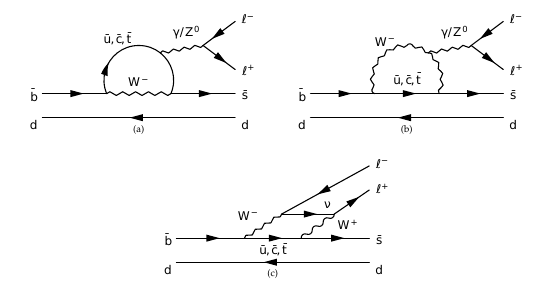
\includegraphics[width=0.8\linewidth]{KstarFeynman}
\caption{Feynman diagrams for decay $B_d$ $\rightarrow$ $\mu^+$ $\mu^-$ at lowest order}
\end{figure}
\end{frame}

\begin{frame}
\frametitle{$B^0$ $\rightarrow$ $K^{*0}$ $\mu$ $\mu$}
three angels define the kinematics of the decay:
\begin{itemize}
  \item ThetaK or $\theta_K$
  \item ThetaL or $\theta_L$
  \item Phi or $\phi$
\end{itemize}

\begin{figure}
  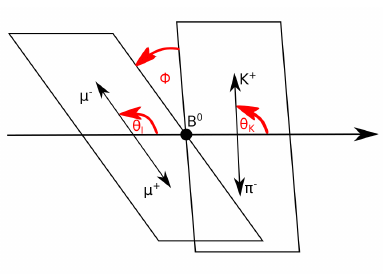
\includegraphics[width=0.6\linewidth]{angels}
  \caption{kinematic variables of the decay $B^0$ $\rightarrow$ $K^{*0}$ $\mu$ $\mu$}
\end{figure}

\end{frame}


\begin{frame}
  \frametitle{classification with Machine Learning (BDT)}
  \begin{itemize}
    \item to eliminate combinatorial background, Boost Decision Trees are used as a black box to classify data into signal and background.
    \item They assign a 'probability' to each event.
    \item sk bdt from the scikit-learn package is used, and uBoost from the hep ml package.
    \item both responses are saved sepratly as one root file.
    \item training is performed on the Linux Cluster in Zurich
  \end{itemize}
\end{frame}

\begin{frame}
  \frametitle{Region to train}
  \begin{itemize}
    \item you want the bdt to train in the background region
    \item J/Psi has two resonance which will be cut off
    \item since a bdt needs real data for training the data is Kfolded. That means that data is splitted into parts to train and to classify.
    \item 10 runs are performed in each 90\% are used for training to classify 10\% in the end all the data is classified. One run is called a fold.
  \end{itemize}

  \begin{figure}
\centering
\begin{subfigure}{0.5\textwidth}
  \centering
  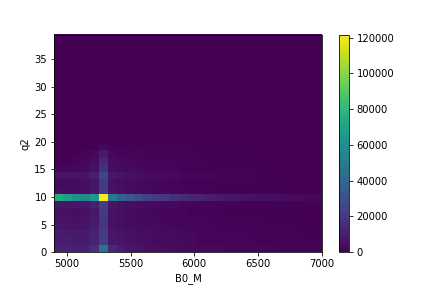
\includegraphics[width=1\linewidth]{beforeCutPlot}
  \caption{Before Cut}
\end{subfigure}%
\begin{subfigure}{0.5\textwidth}
  \centering
  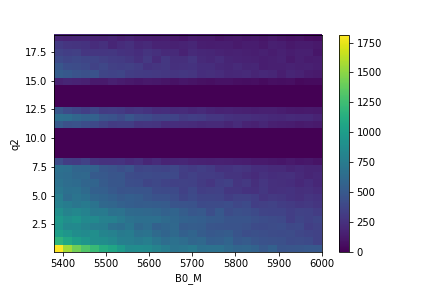
\includegraphics[width=1\linewidth]{cutPlot}
  \caption{After Cut}
\end{subfigure}
\end{figure}

\end{frame}

\begin{frame}
  \frametitle{training of the BDTs}
  8 train parameters:
  \begin{itemize}
    \item B0 P
    \item B0 PT
    \item B0 ENDVERTEX CHI2
    \item B0 IP OWNPV
    \item B0 IPCHI2 OWNPV
    \item B0 FD OWNPV
    \item B0 FDCHI2 OWNPV
    \item B0 relinfo VTXISOBDTHARDFIRSTVALUE
  \end{itemize}
  4 uniform parameters:
  \begin{itemize}
    \item B0 M
    \item B0 ThetaK
    \item B0 ThetaL
    \item B0 Phi
  \end{itemize}
  uniform parameters have to be uncorrelated. \\
  But BDT might find a correlation which is bad.
\end{frame}

% \begin{frame}
%   \frametitle{BDT correlation check}
%
%   \begin{figure}
%   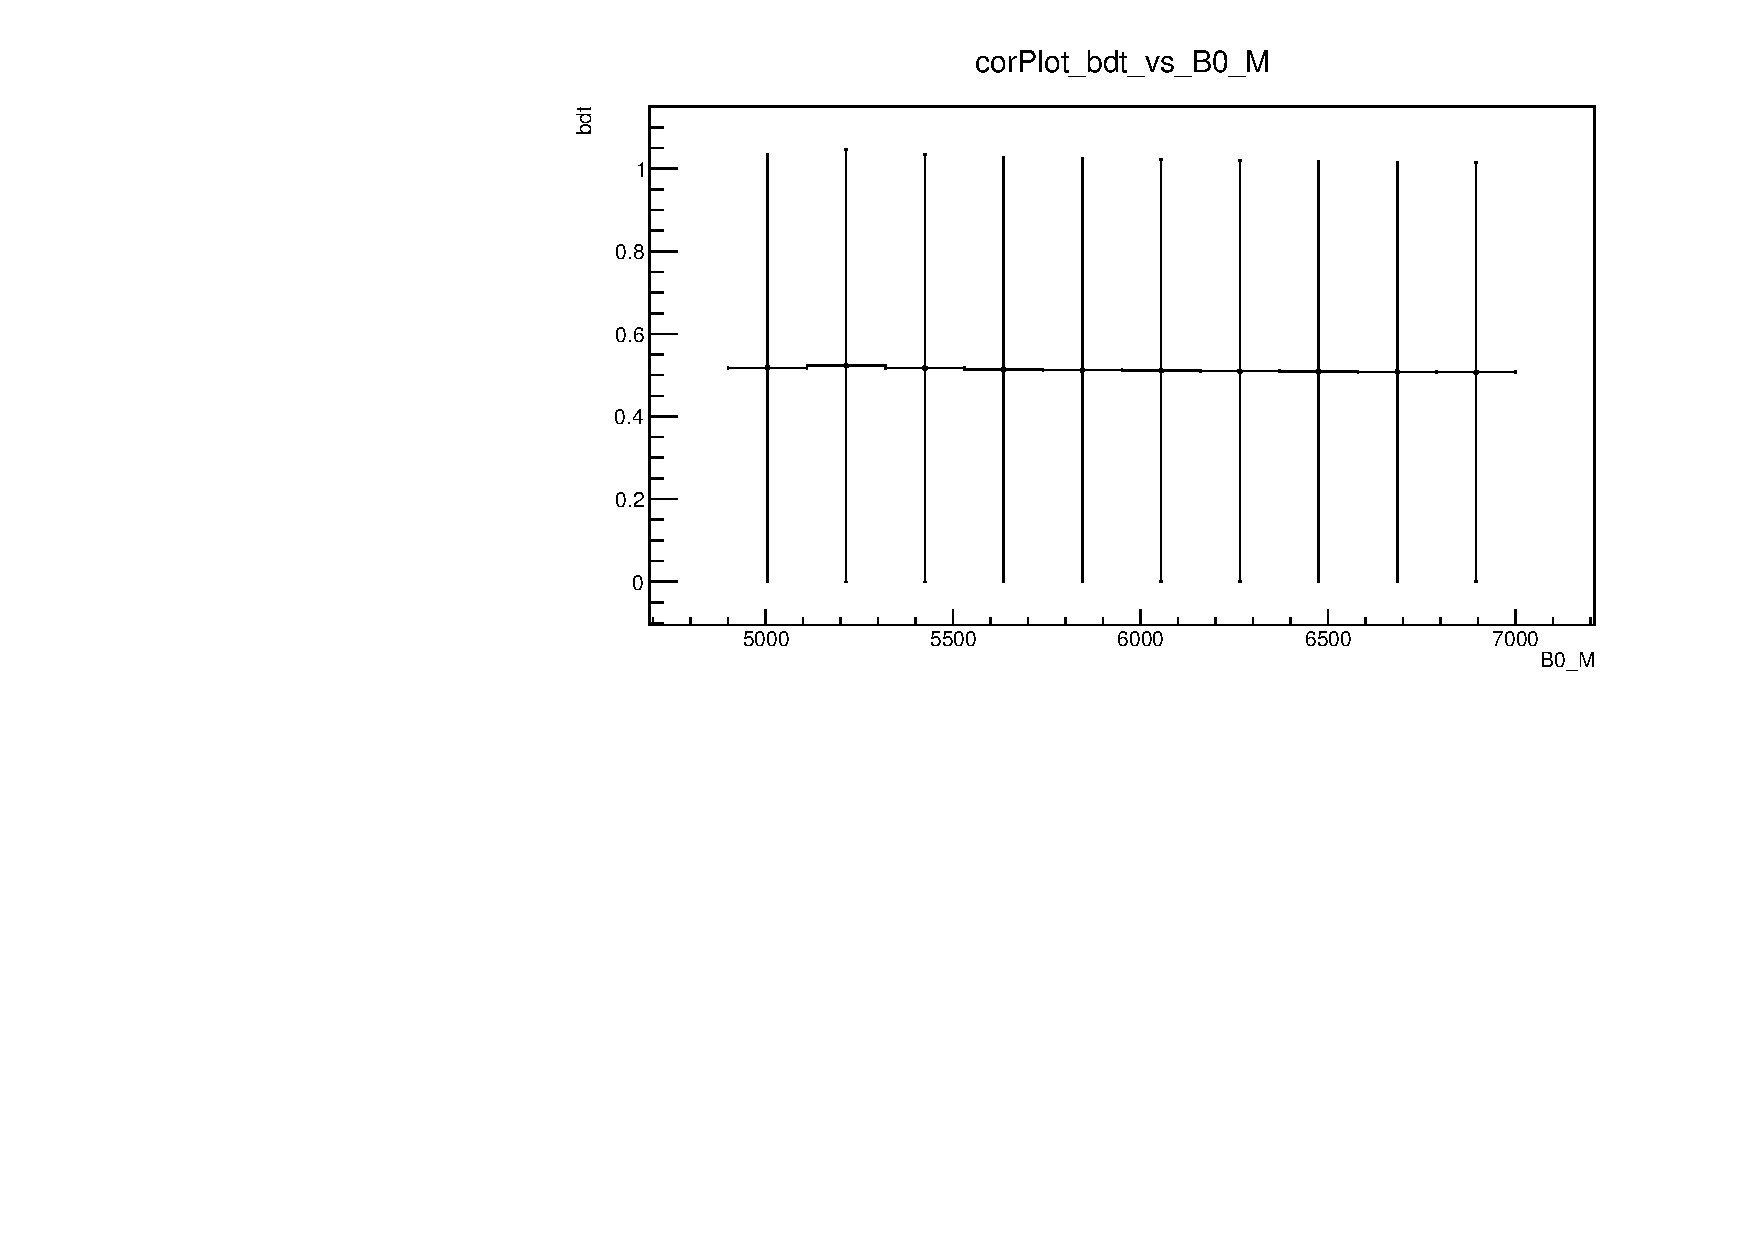
\includegraphics[width=1.0\linewidth]{plots/corPlot_bdt_vs_B0_M.pdf}
%   \end{figure}
%
% \end{frame}
%
% \begin{frame}
%   \frametitle{BDT correlation check}

%   \begin{figure}
%   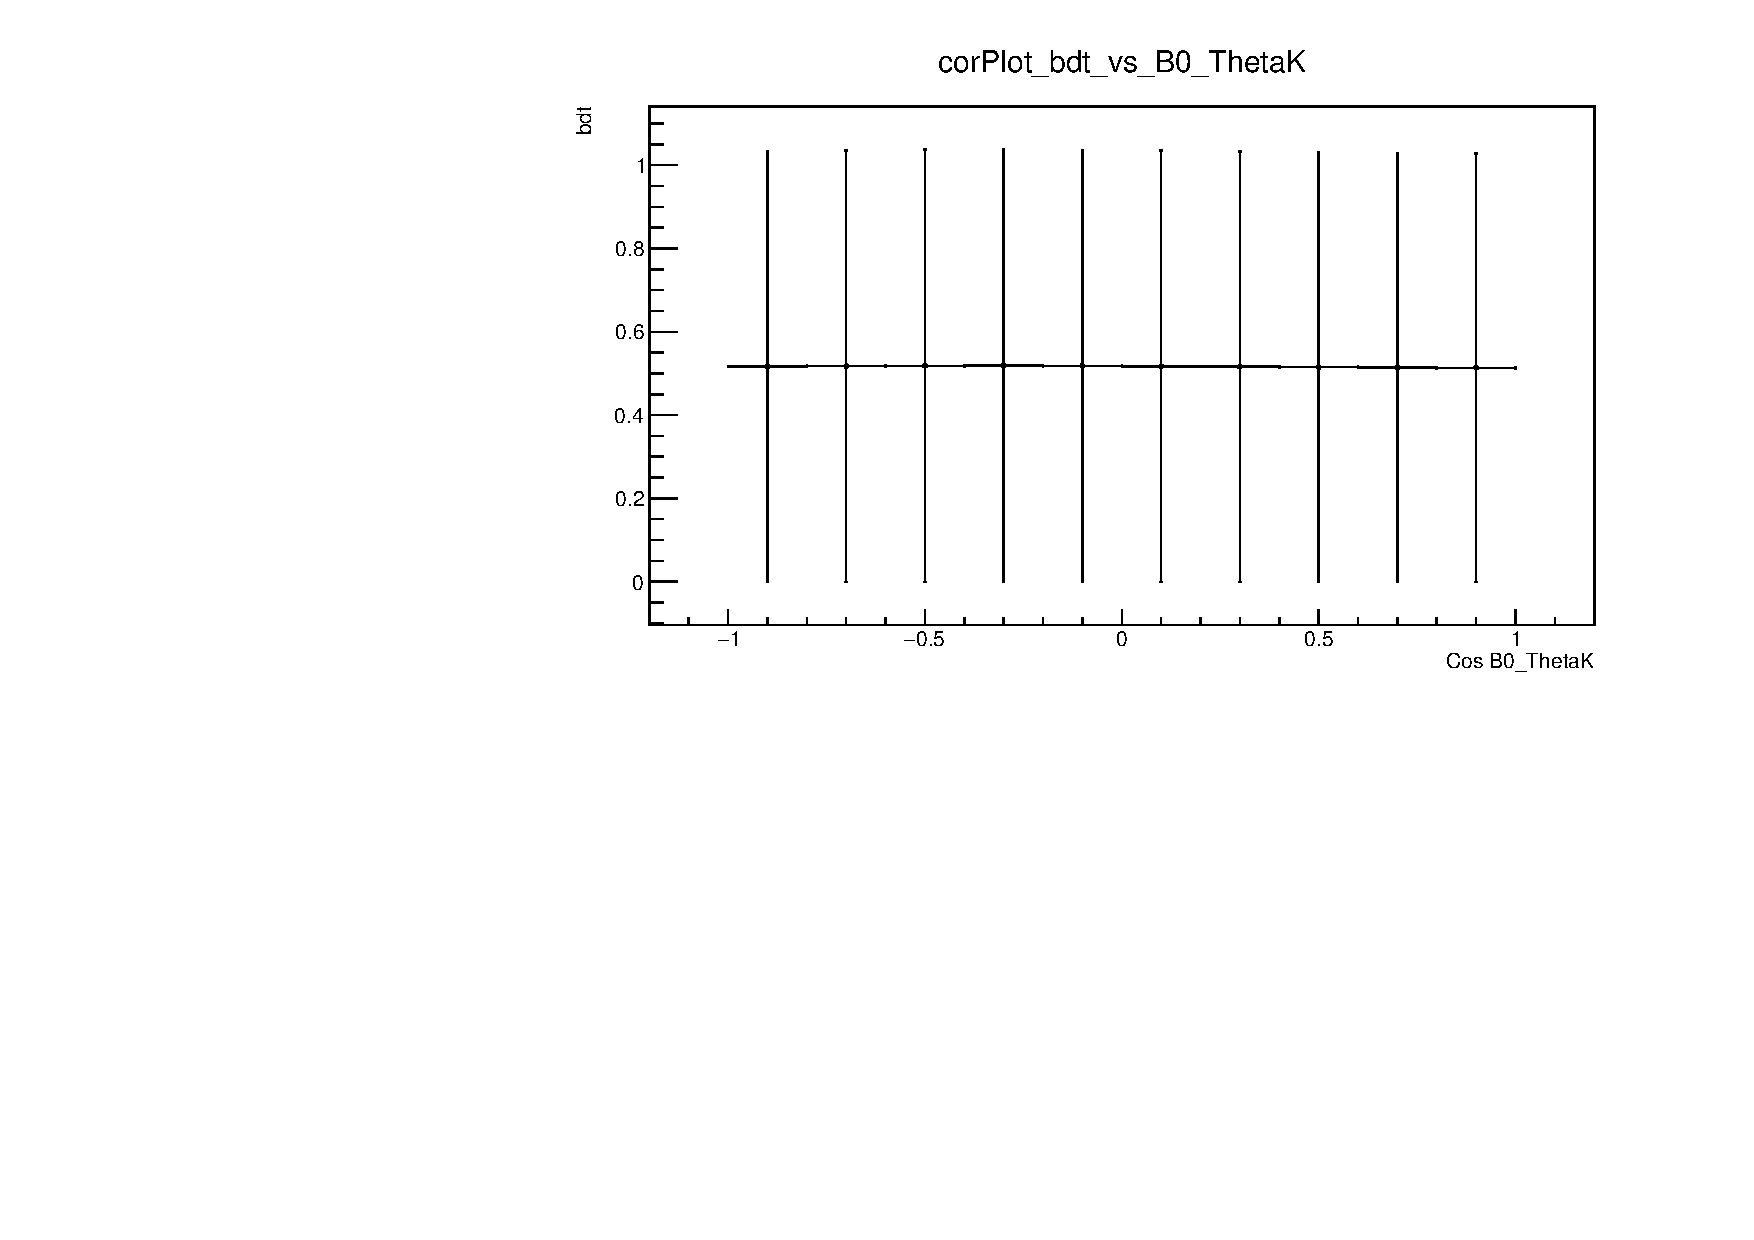
\includegraphics[width=1.0\linewidth]{plots/corPlot_bdt_vs_B0_ThetaK.pdf}
%   \end{figure}
%
% \end{frame}
%
% \begin{frame}
%   \frametitle{BDT correlation check}
%
%   \begin{figure}
%   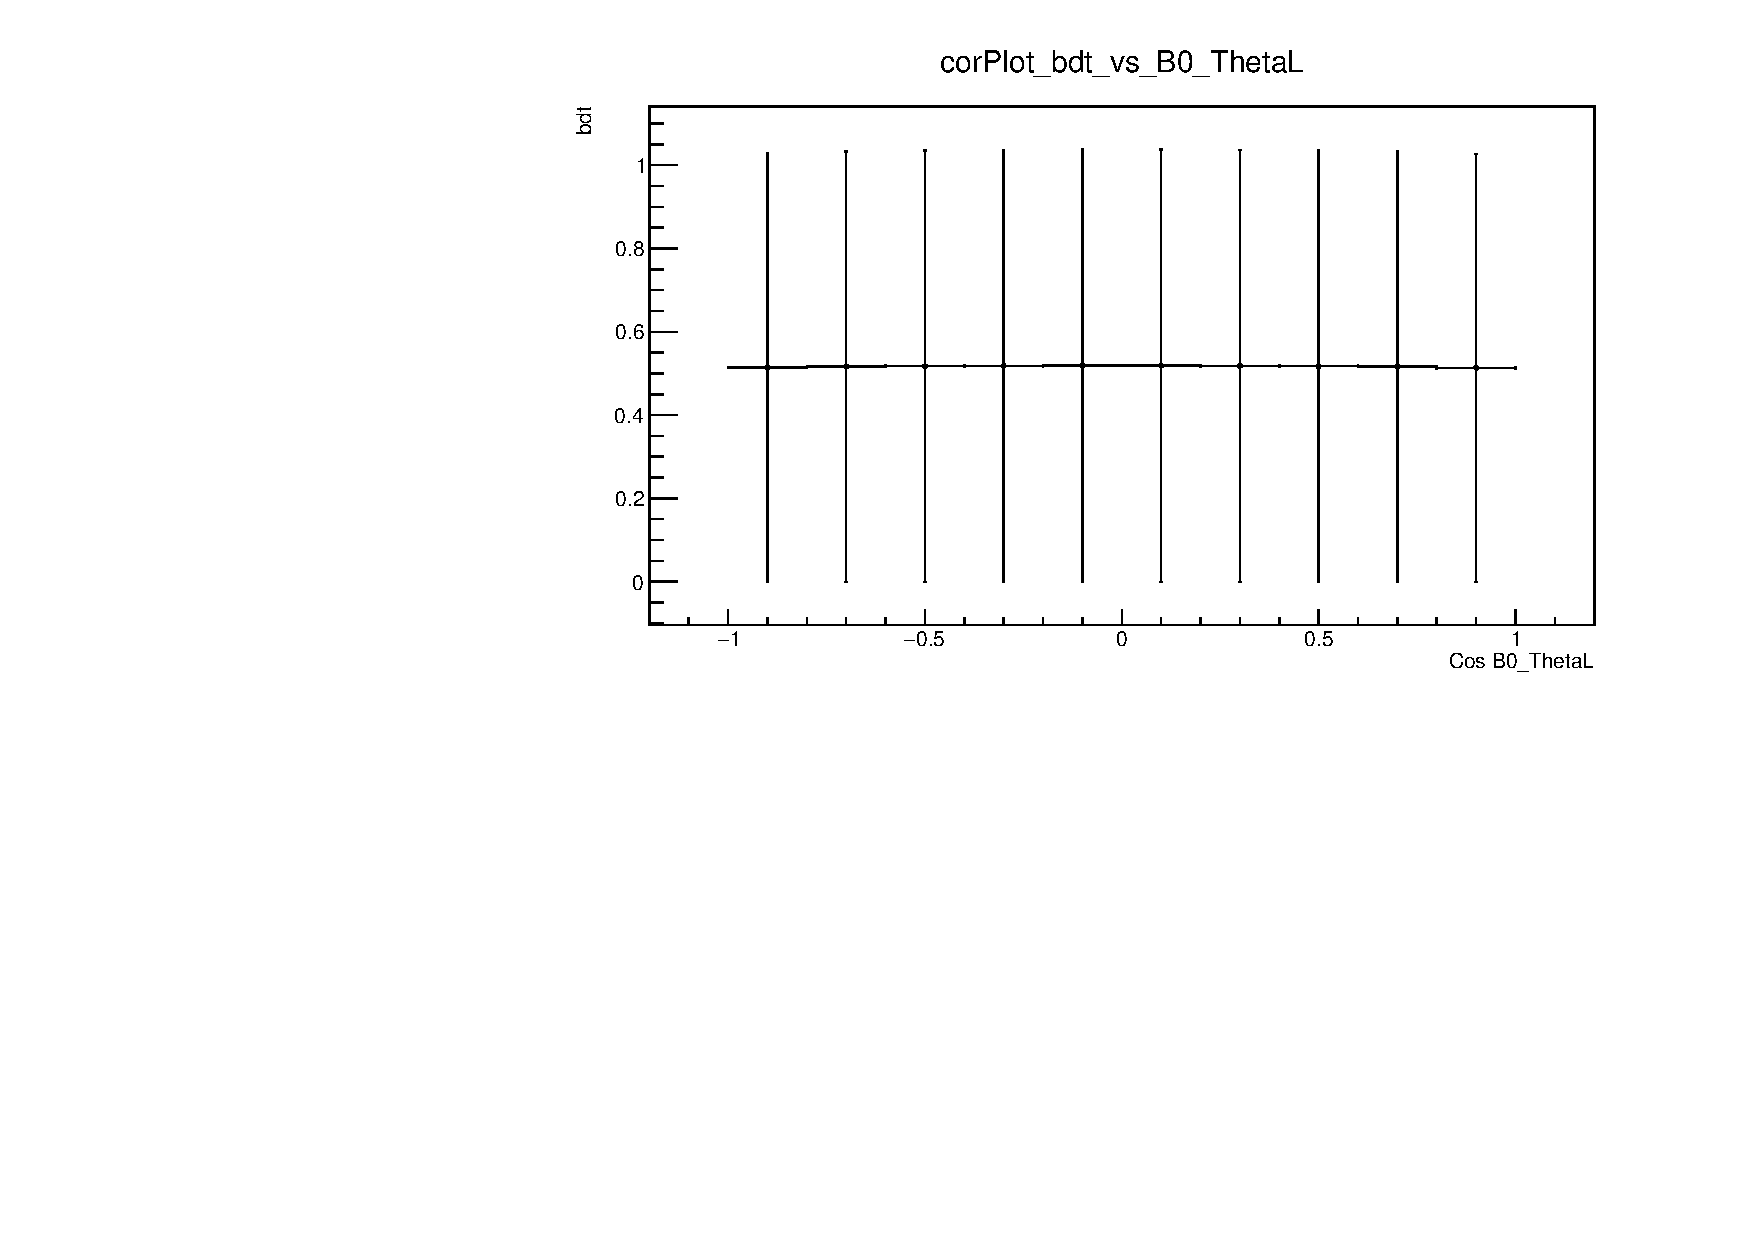
\includegraphics[width=1.0\linewidth]{plots/corPlot_bdt_vs_B0_ThetaL.pdf}
%   \end{figure}
%
% \end{frame}

\begin{frame}
\frametitle{BDT correlation check}
If there is no correlation this plot, between the bdt response and one of the uniform parameters, is flat.
Therefore is no correlation between the sk bdt and the B0 mass. There is just a very small correlation between uBoost and the B0 mass.
 \begin{figure}
 \centering
 \begin{subfigure}{0.5\textwidth}
 \centering
 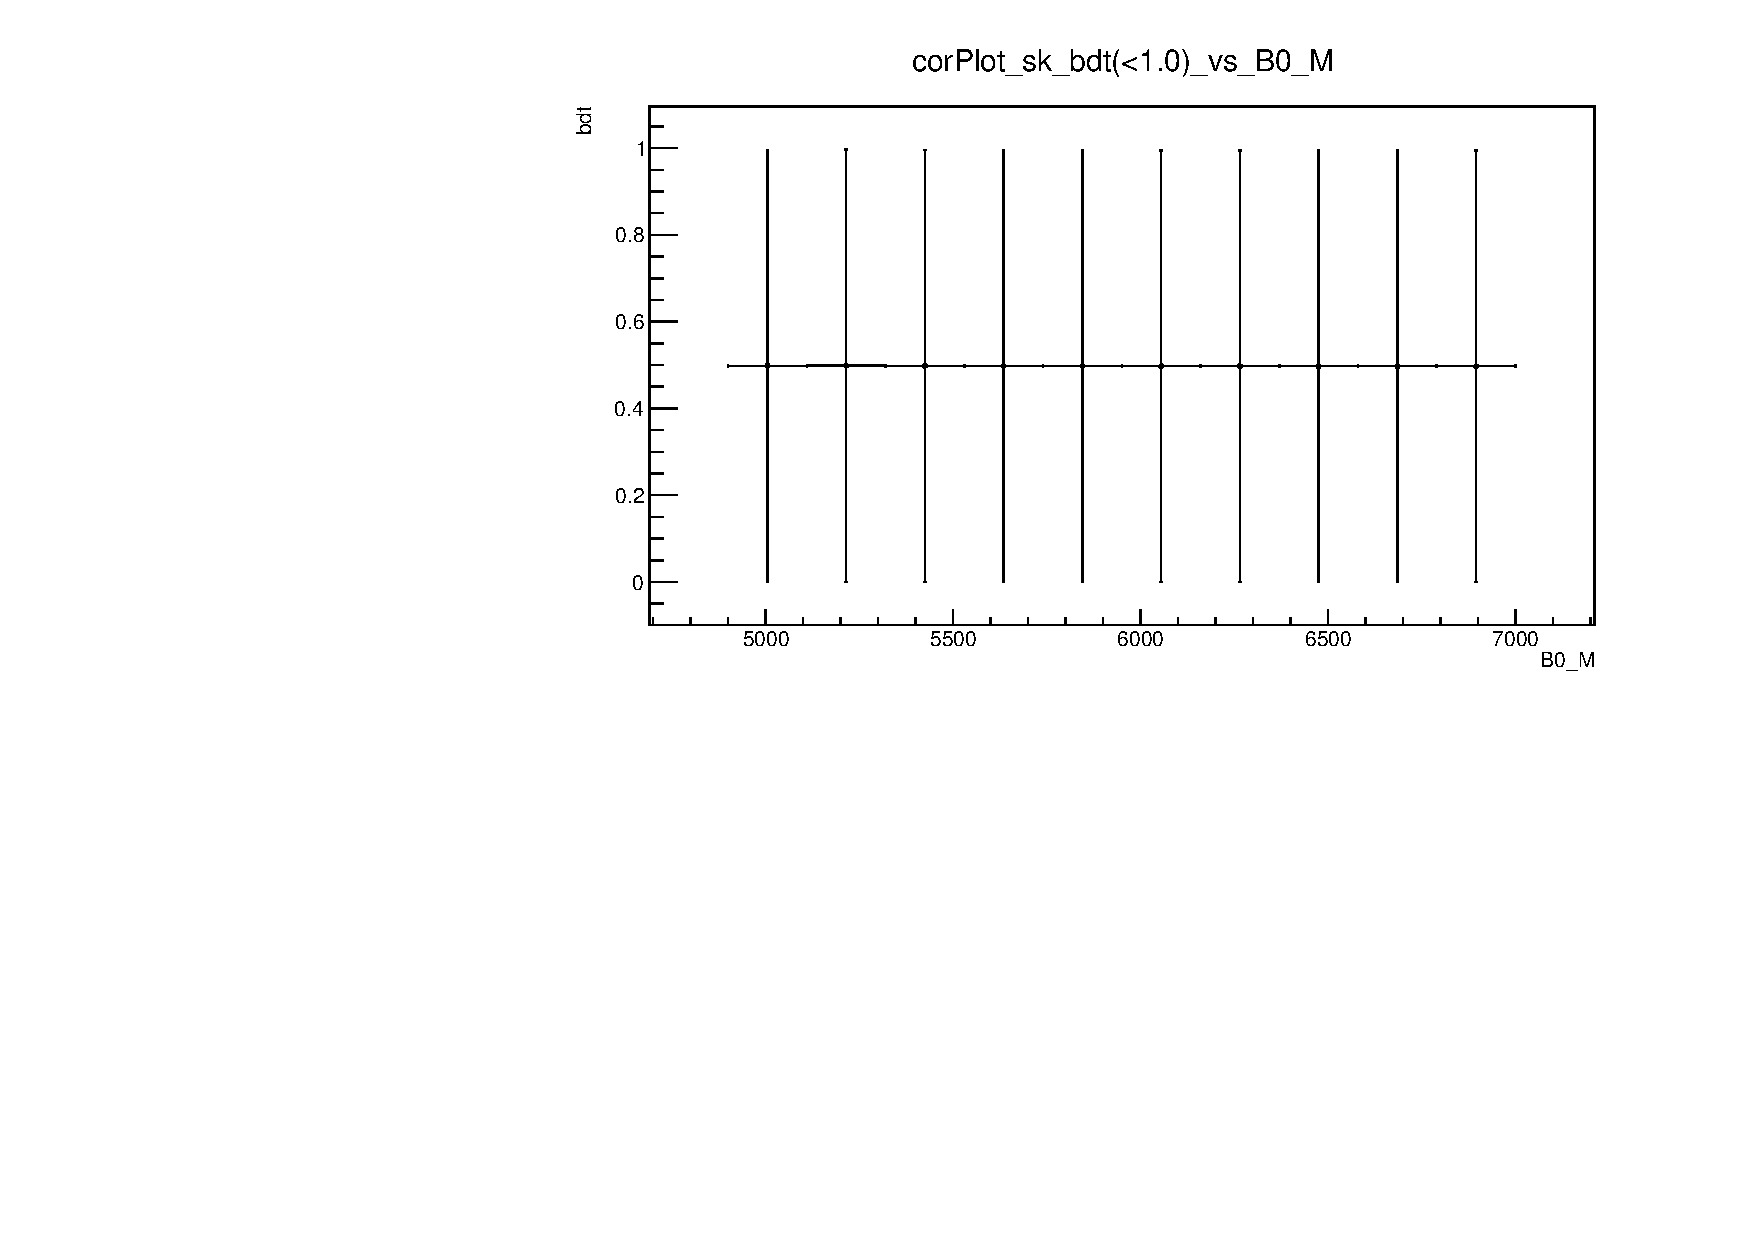
\includegraphics[width=1.0\linewidth]{plots/corPlot_sk_bdt(<1.0)_vs_B0_M.pdf}
 \caption{Correlation sk bdt VS B0 M}
 \end{subfigure}%
\begin{subfigure}{0.5\textwidth}
\centering
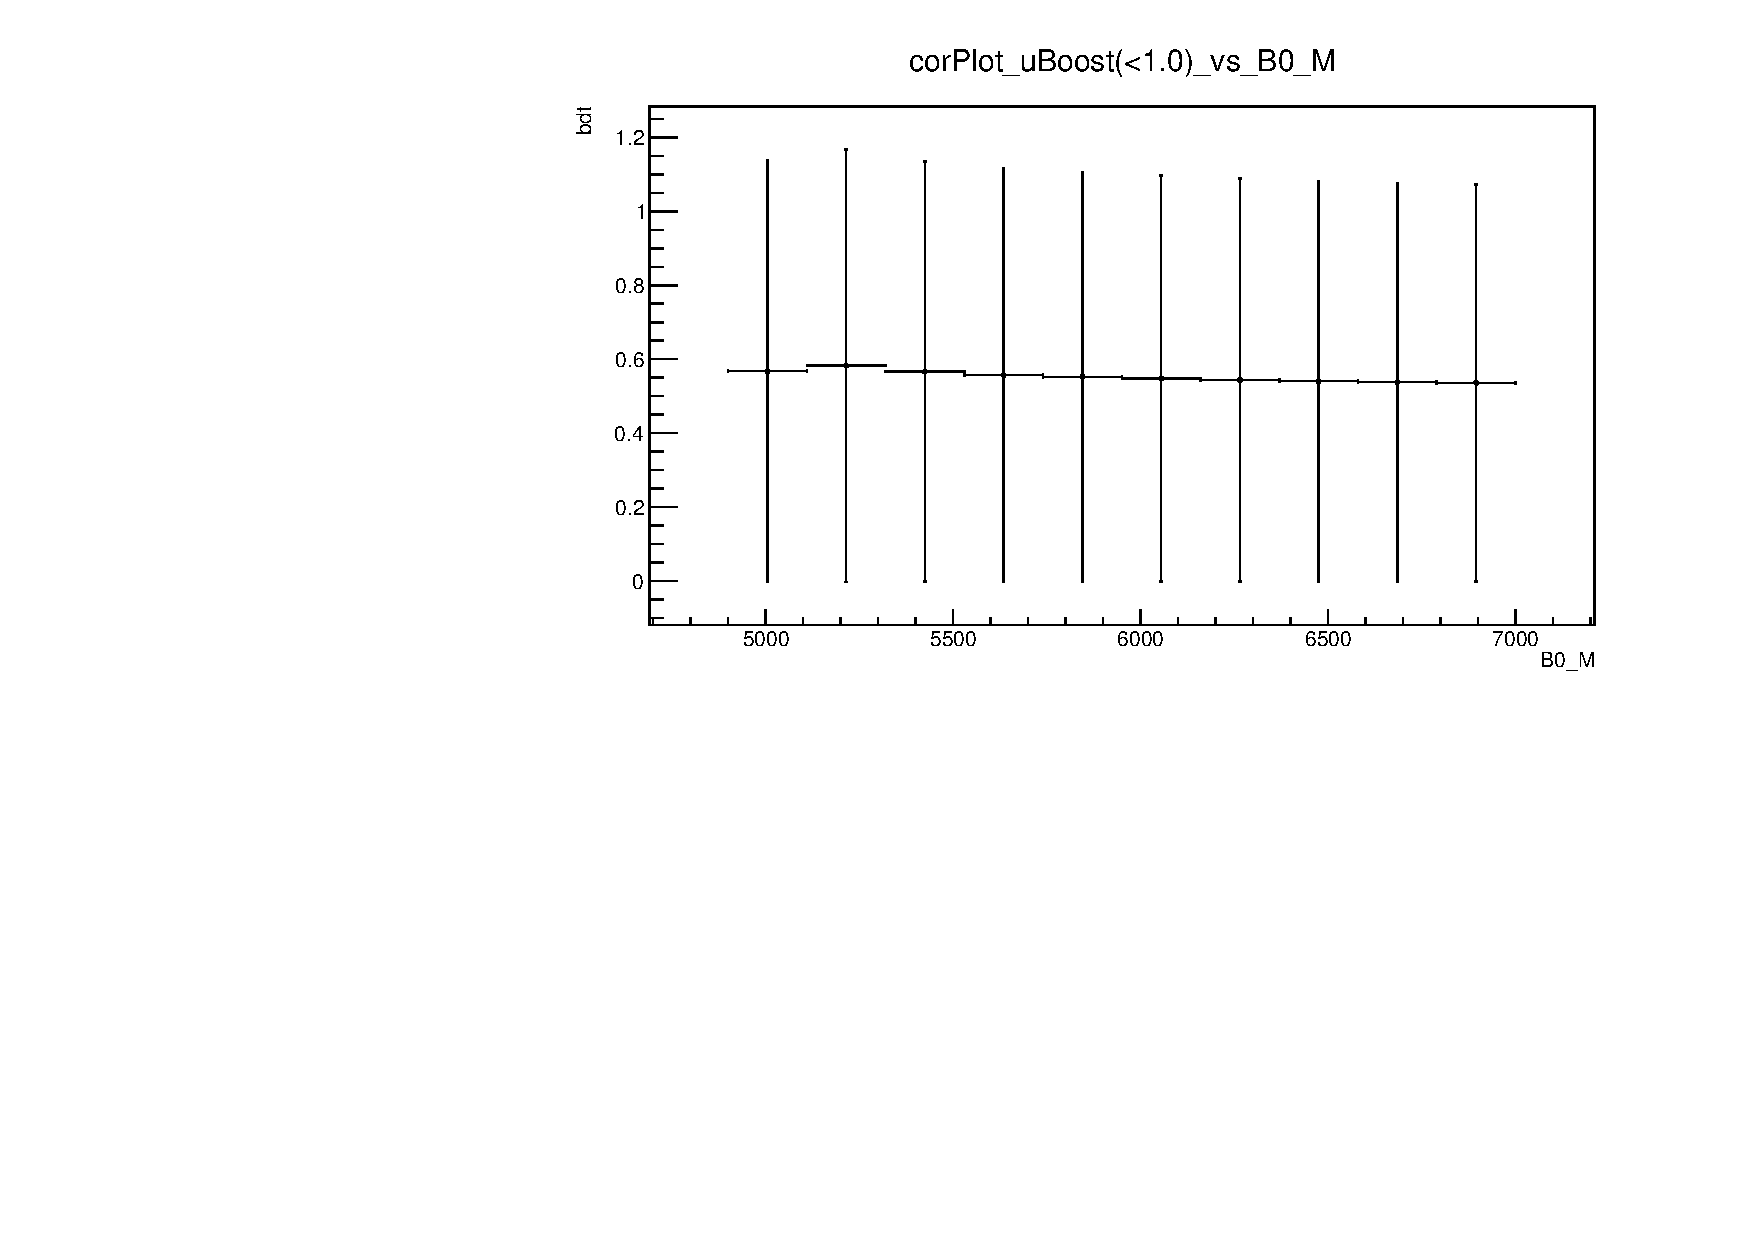
\includegraphics[width=1.0\linewidth]{plots/corPlot_uBoost(<1.0)_vs_B0_M.pdf}
\caption{Correlation uBoost VS B0 M}
\end{subfigure}
\end{figure}
\end{frame}

\begin{frame}
\frametitle{BDT correlation check}
There is no correlation between the bdts and the cosine of the ThetaK angle.
 \begin{figure}
 \centering
 \begin{subfigure}{0.5\textwidth}
 \centering
 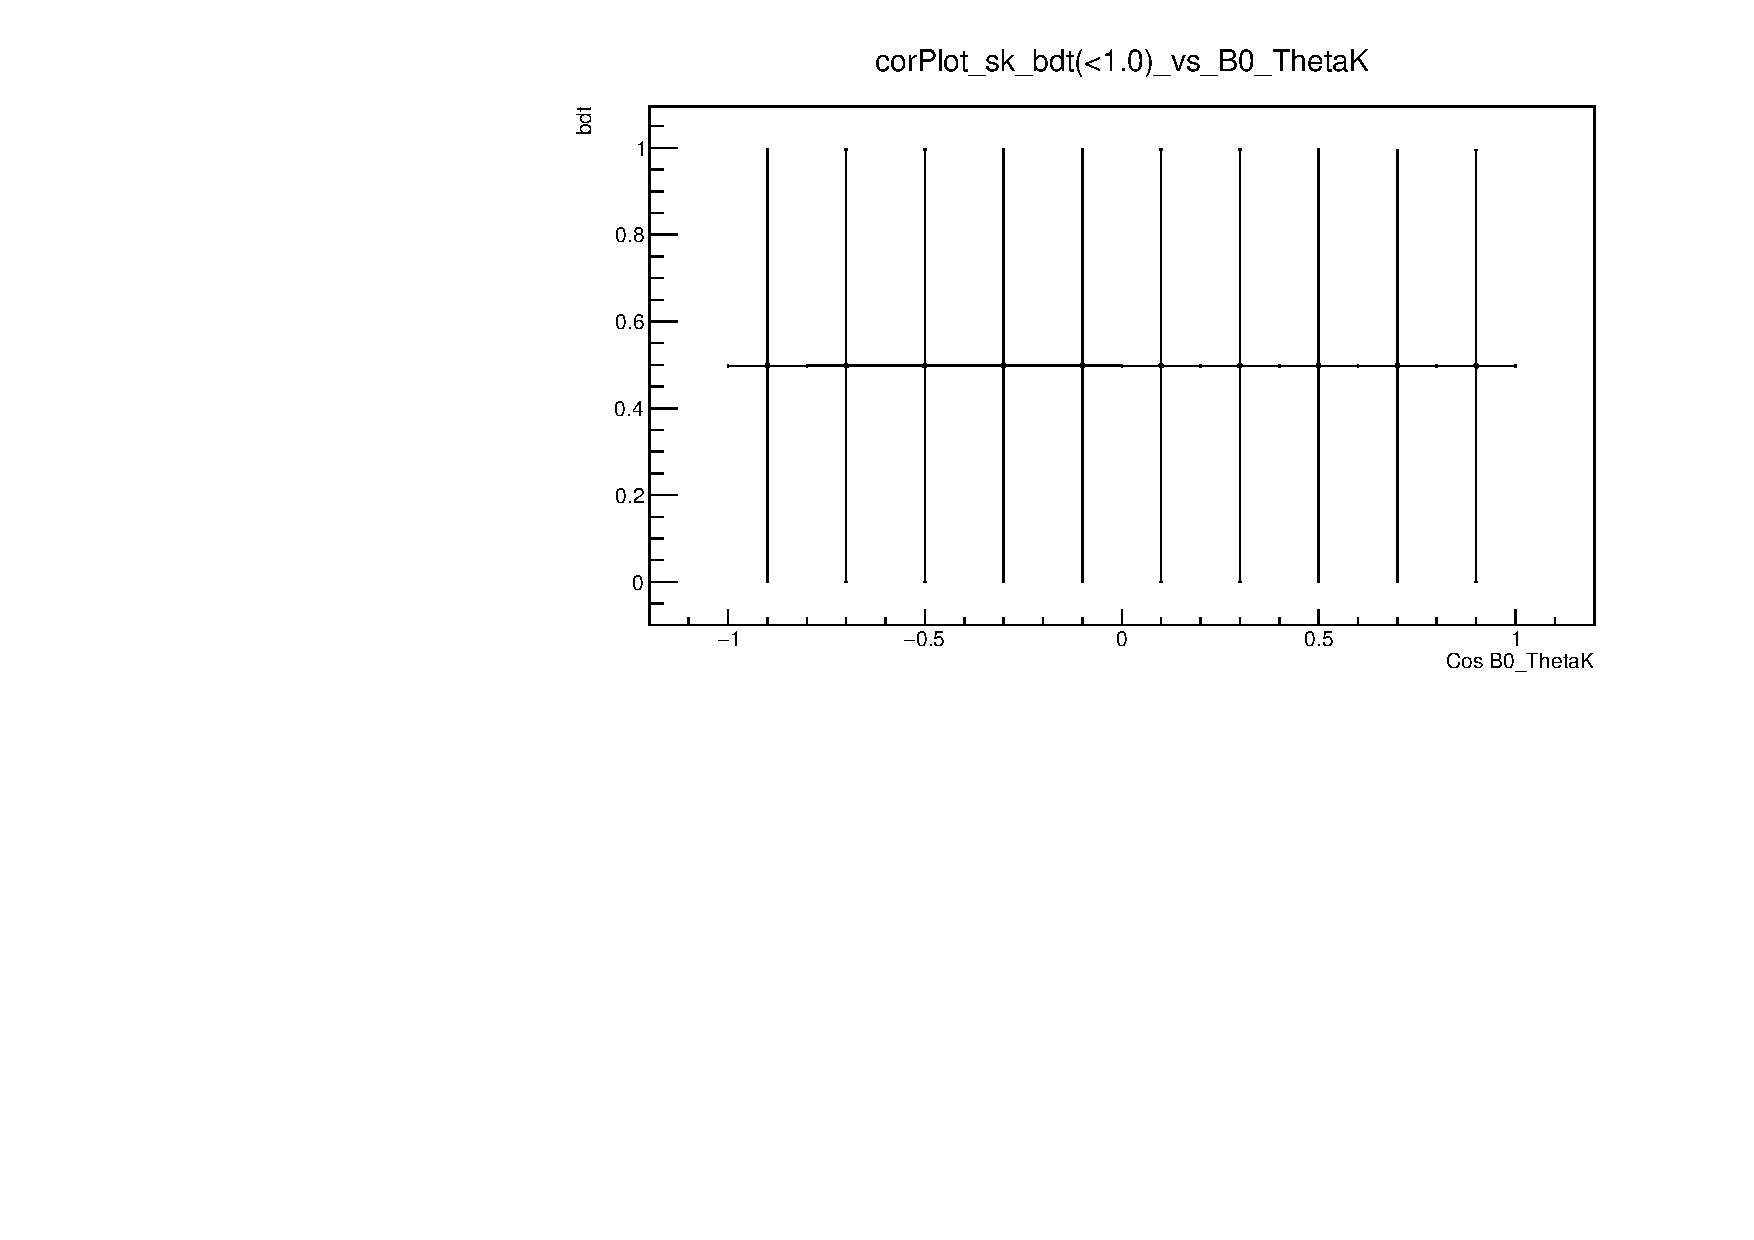
\includegraphics[width=1.0\linewidth]{plots/corPlot_sk_bdt(<1.0)_vs_B0_ThetaK.pdf}
 \caption{Correlation sk bdt VS B0 ThetaK}
 \end{subfigure}%
\begin{subfigure}{0.5\textwidth}
\centering
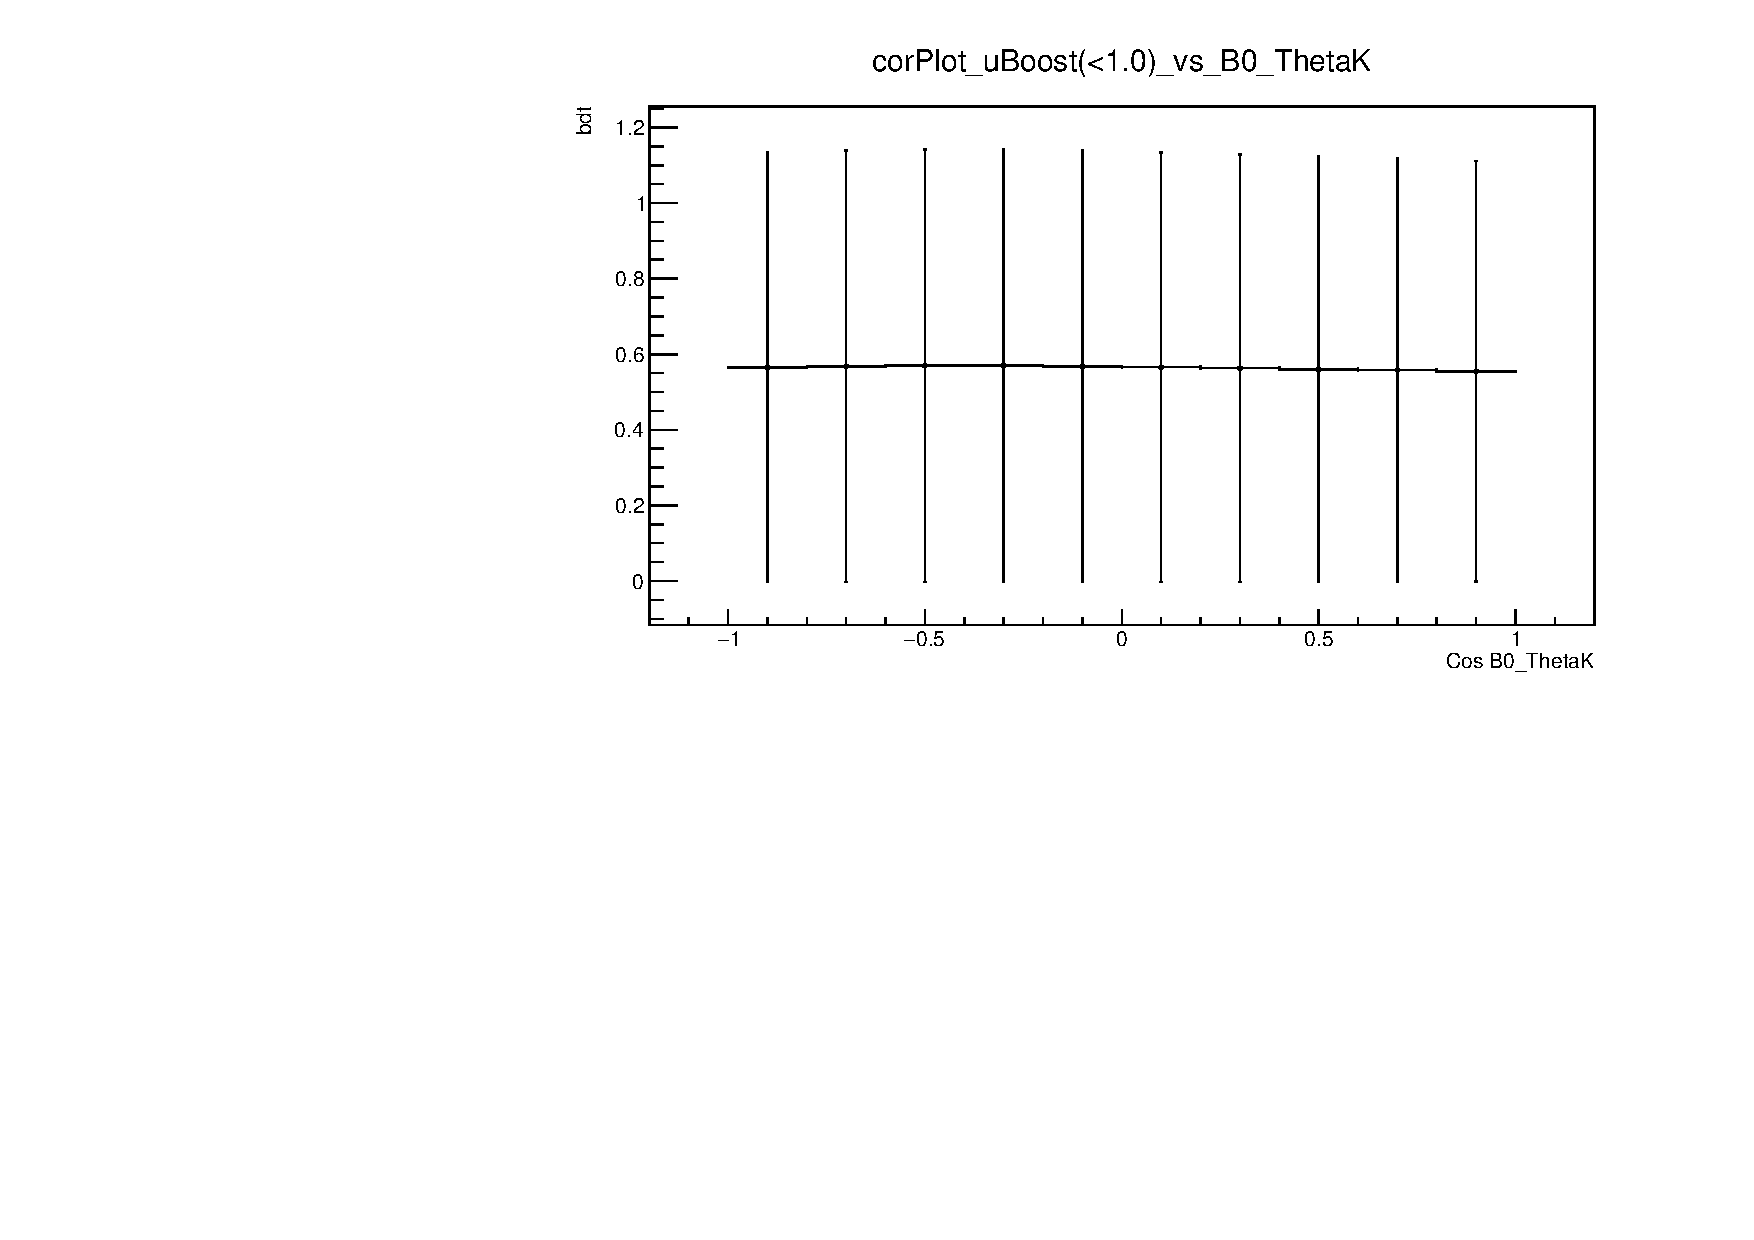
\includegraphics[width=1.0\linewidth]{plots/corPlot_uBoost(<1.0)_vs_B0_ThetaK.pdf}
\caption{Correlation uBoost VS B0 ThetaK}
\end{subfigure}
\end{figure}
\end{frame}

\begin{frame}
\frametitle{BDT correlation check}
There is no correlation between the bdts and the cosine of the ThetaL angle.
 \begin{figure}
 \centering
 \begin{subfigure}{0.5\textwidth}
 \centering
 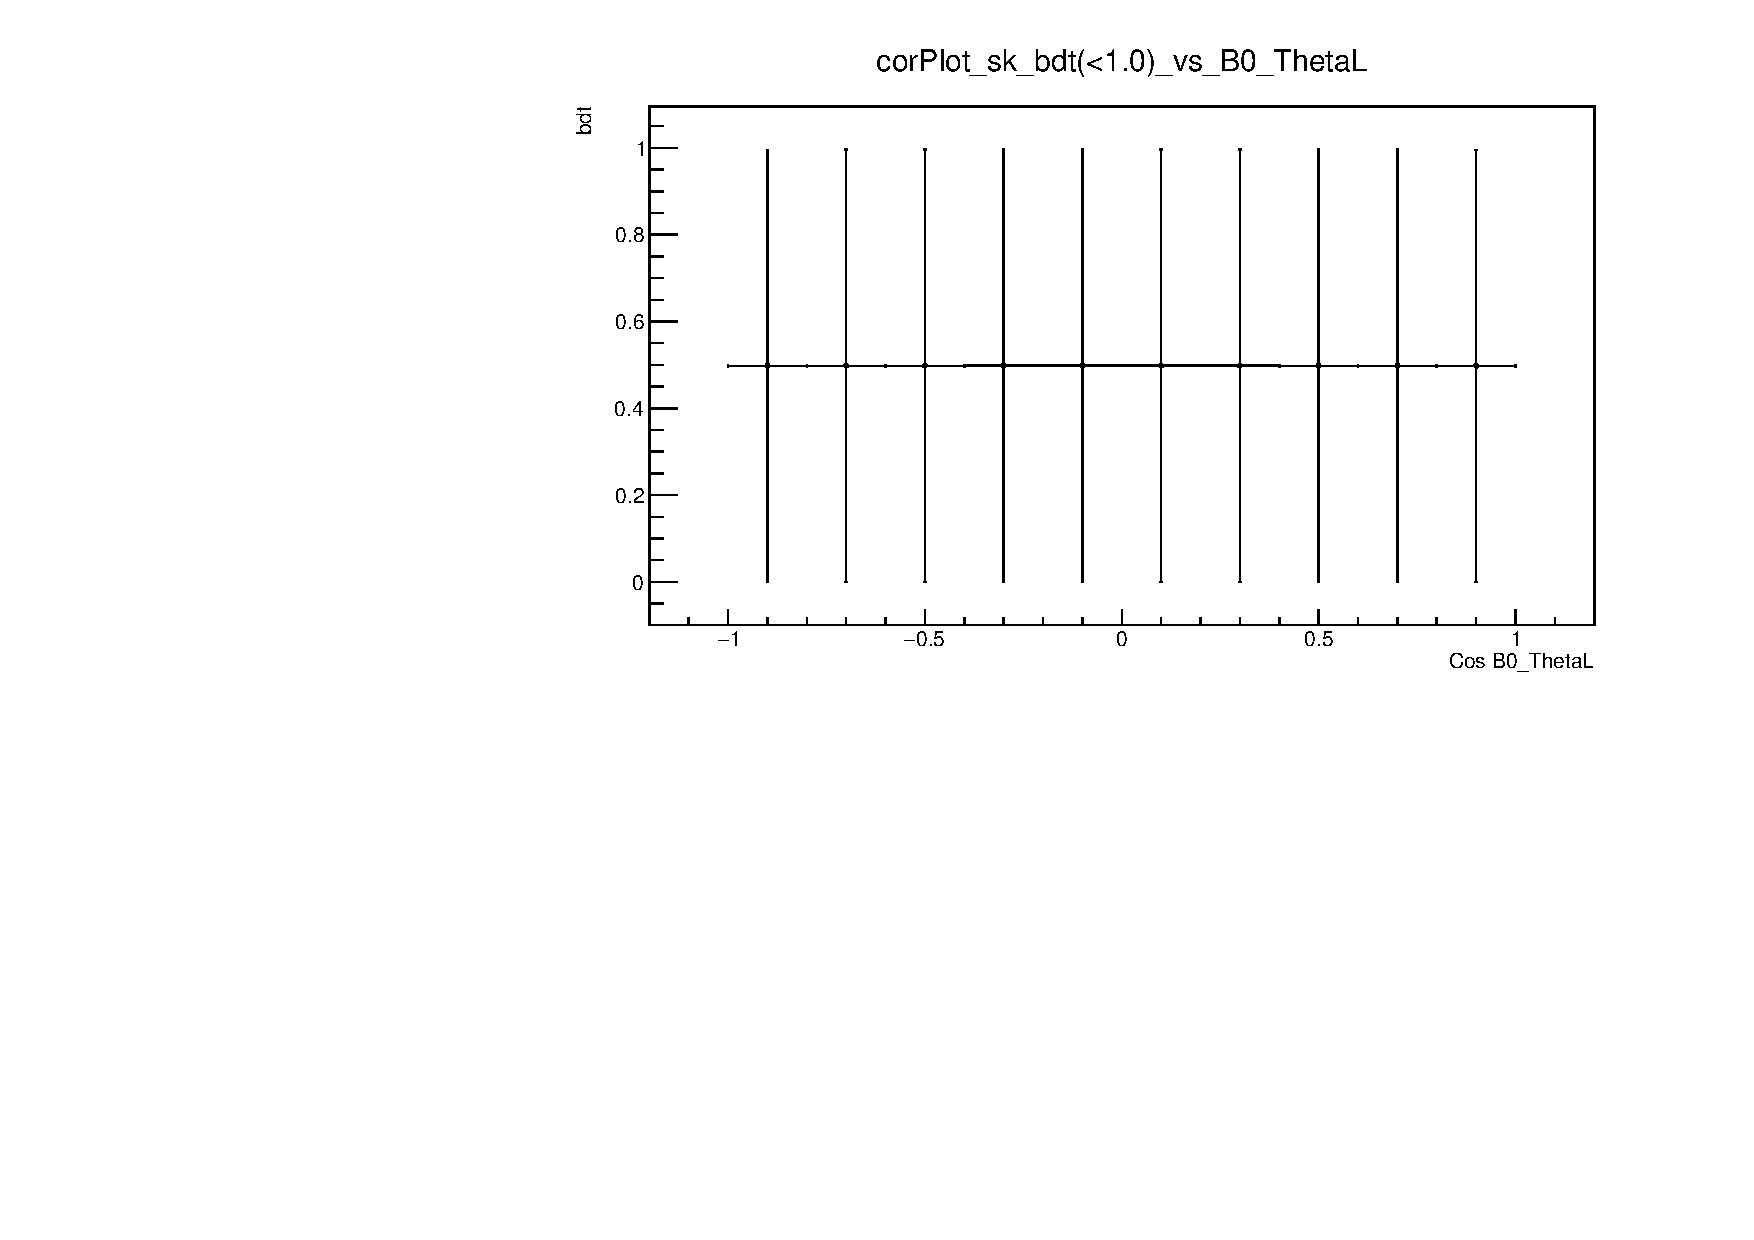
\includegraphics[width=1.0\linewidth]{plots/corPlot_sk_bdt(<1.0)_vs_B0_ThetaL.pdf}
 \caption{Correlation sk bdt VS B0 ThetaL}
 \end{subfigure}%
\begin{subfigure}{0.5\textwidth}
\centering
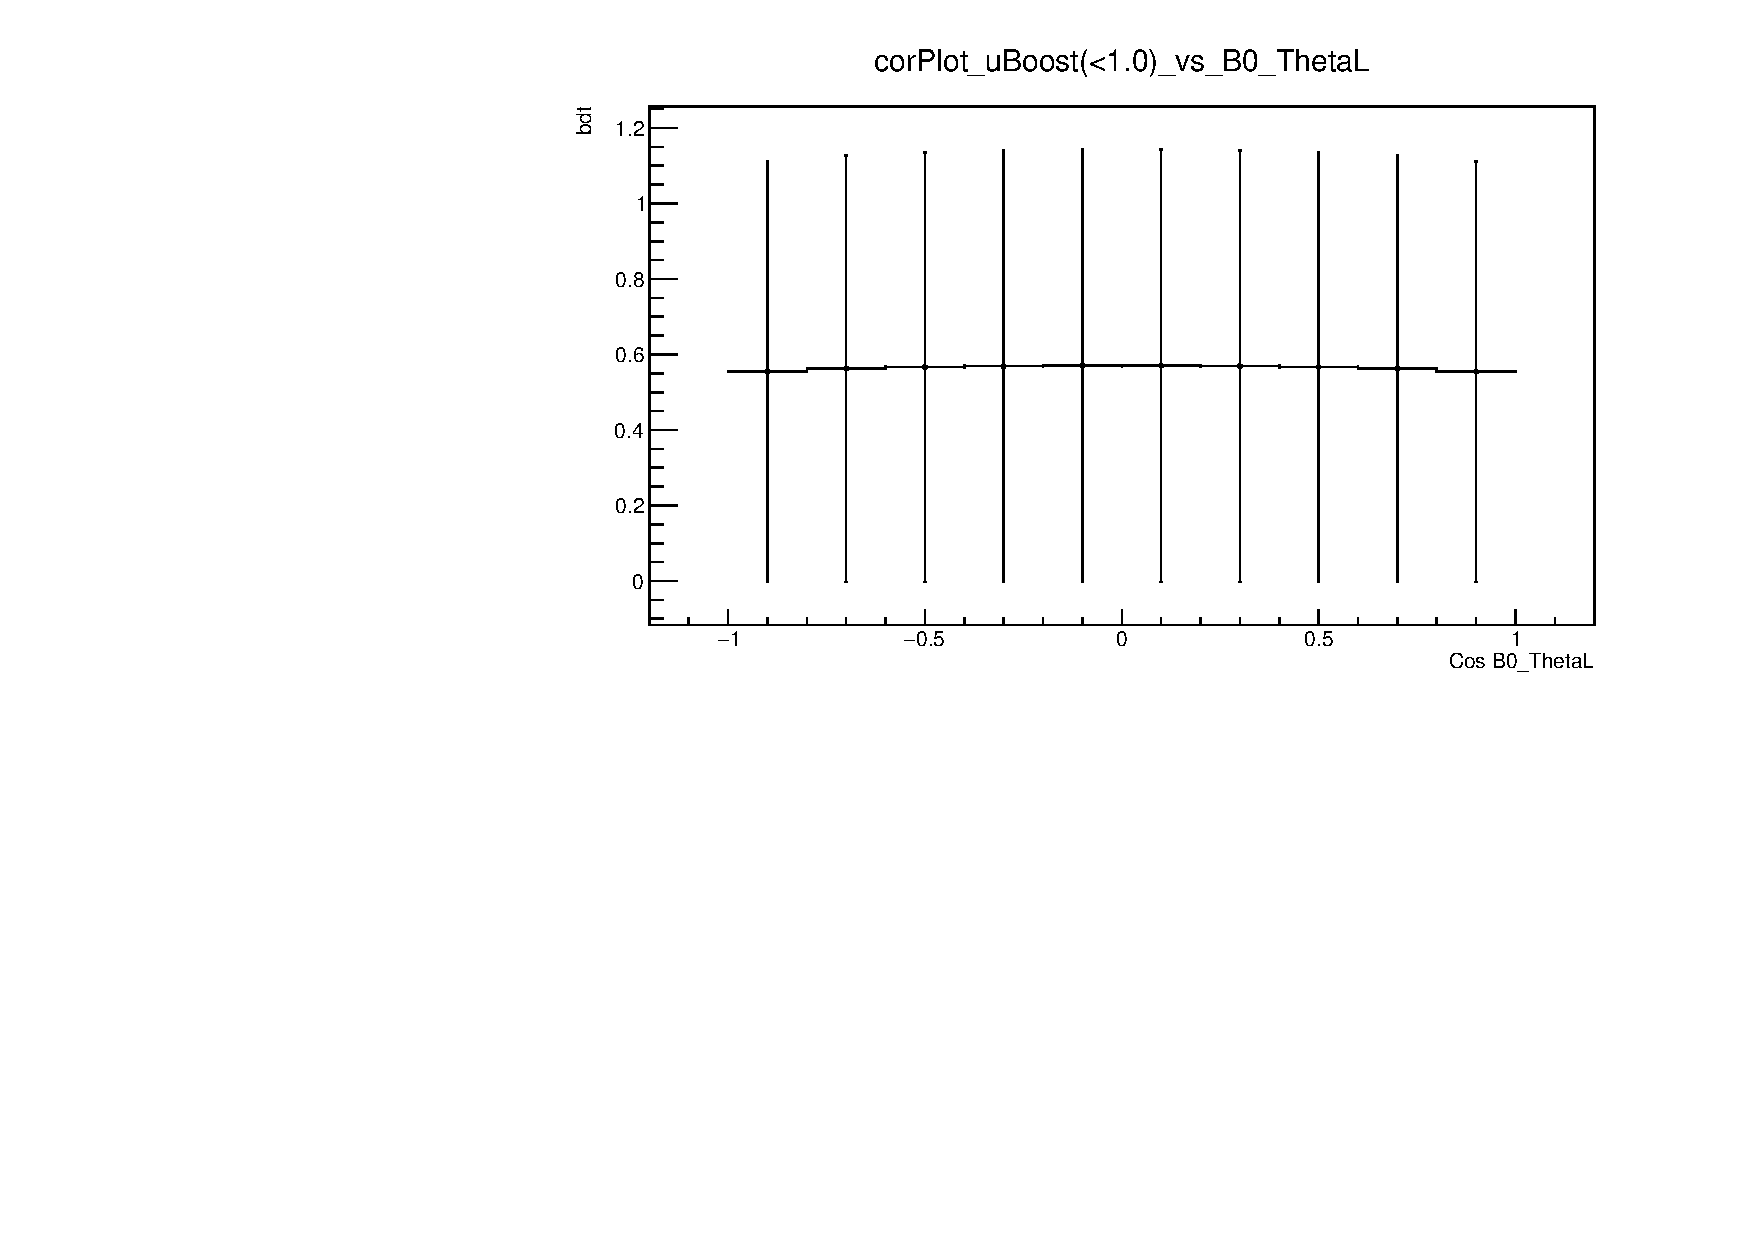
\includegraphics[width=1.0\linewidth]{plots/corPlot_uBoost(<1.0)_vs_B0_ThetaL.pdf}
\caption{Correlation uBoost VS B0 ThetaL}
\end{subfigure}
\end{figure}
\end{frame}

\begin{frame}
\frametitle{BDT correlation check}
There is no correlation between the bdts and Phi angle.
 \begin{figure}
 \centering
 \begin{subfigure}{0.5\textwidth}
 \centering
 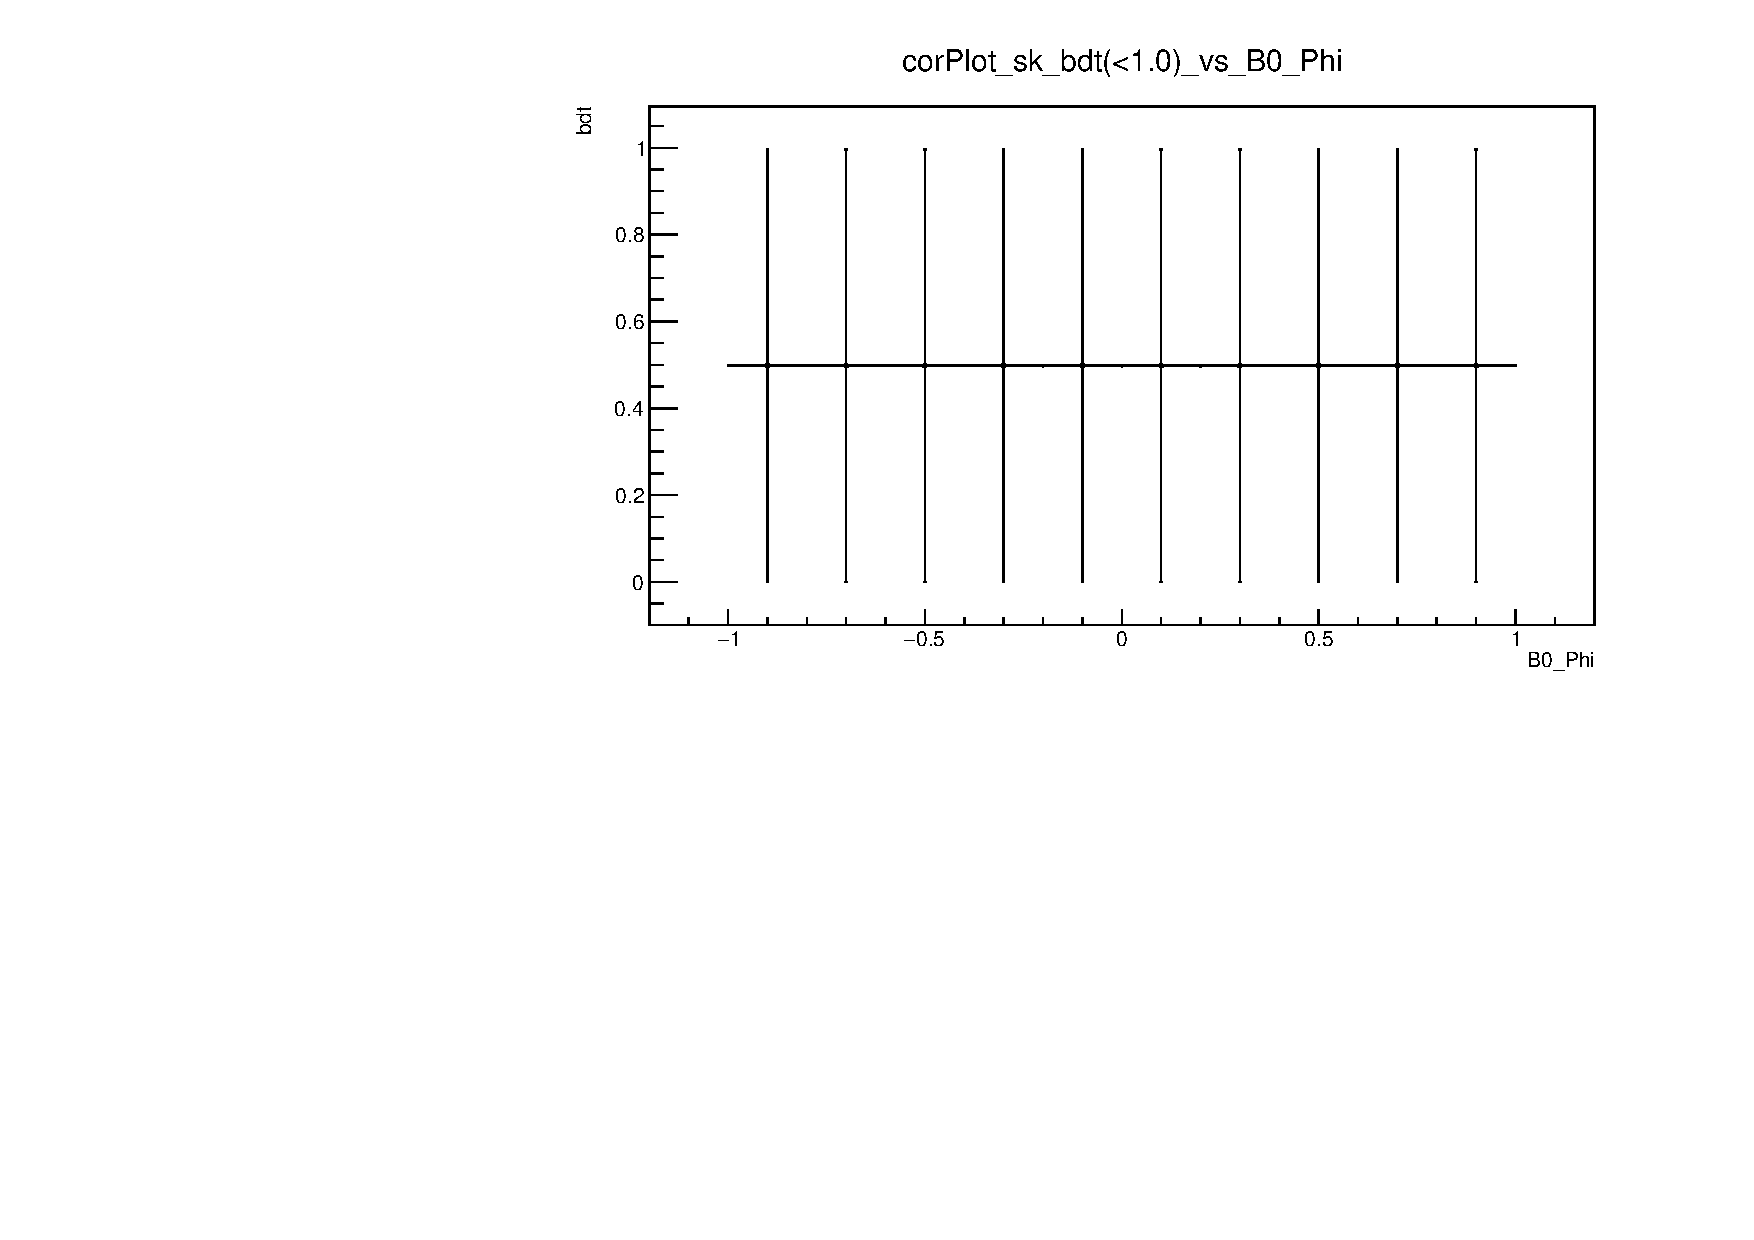
\includegraphics[width=1.0\linewidth]{plots/corPlot_sk_bdt(<1.0)_vs_B0_Phi.pdf}
 \caption{Correlation sk bdt VS B0 Phi}
 \end{subfigure}%
\begin{subfigure}{0.5\textwidth}
\centering
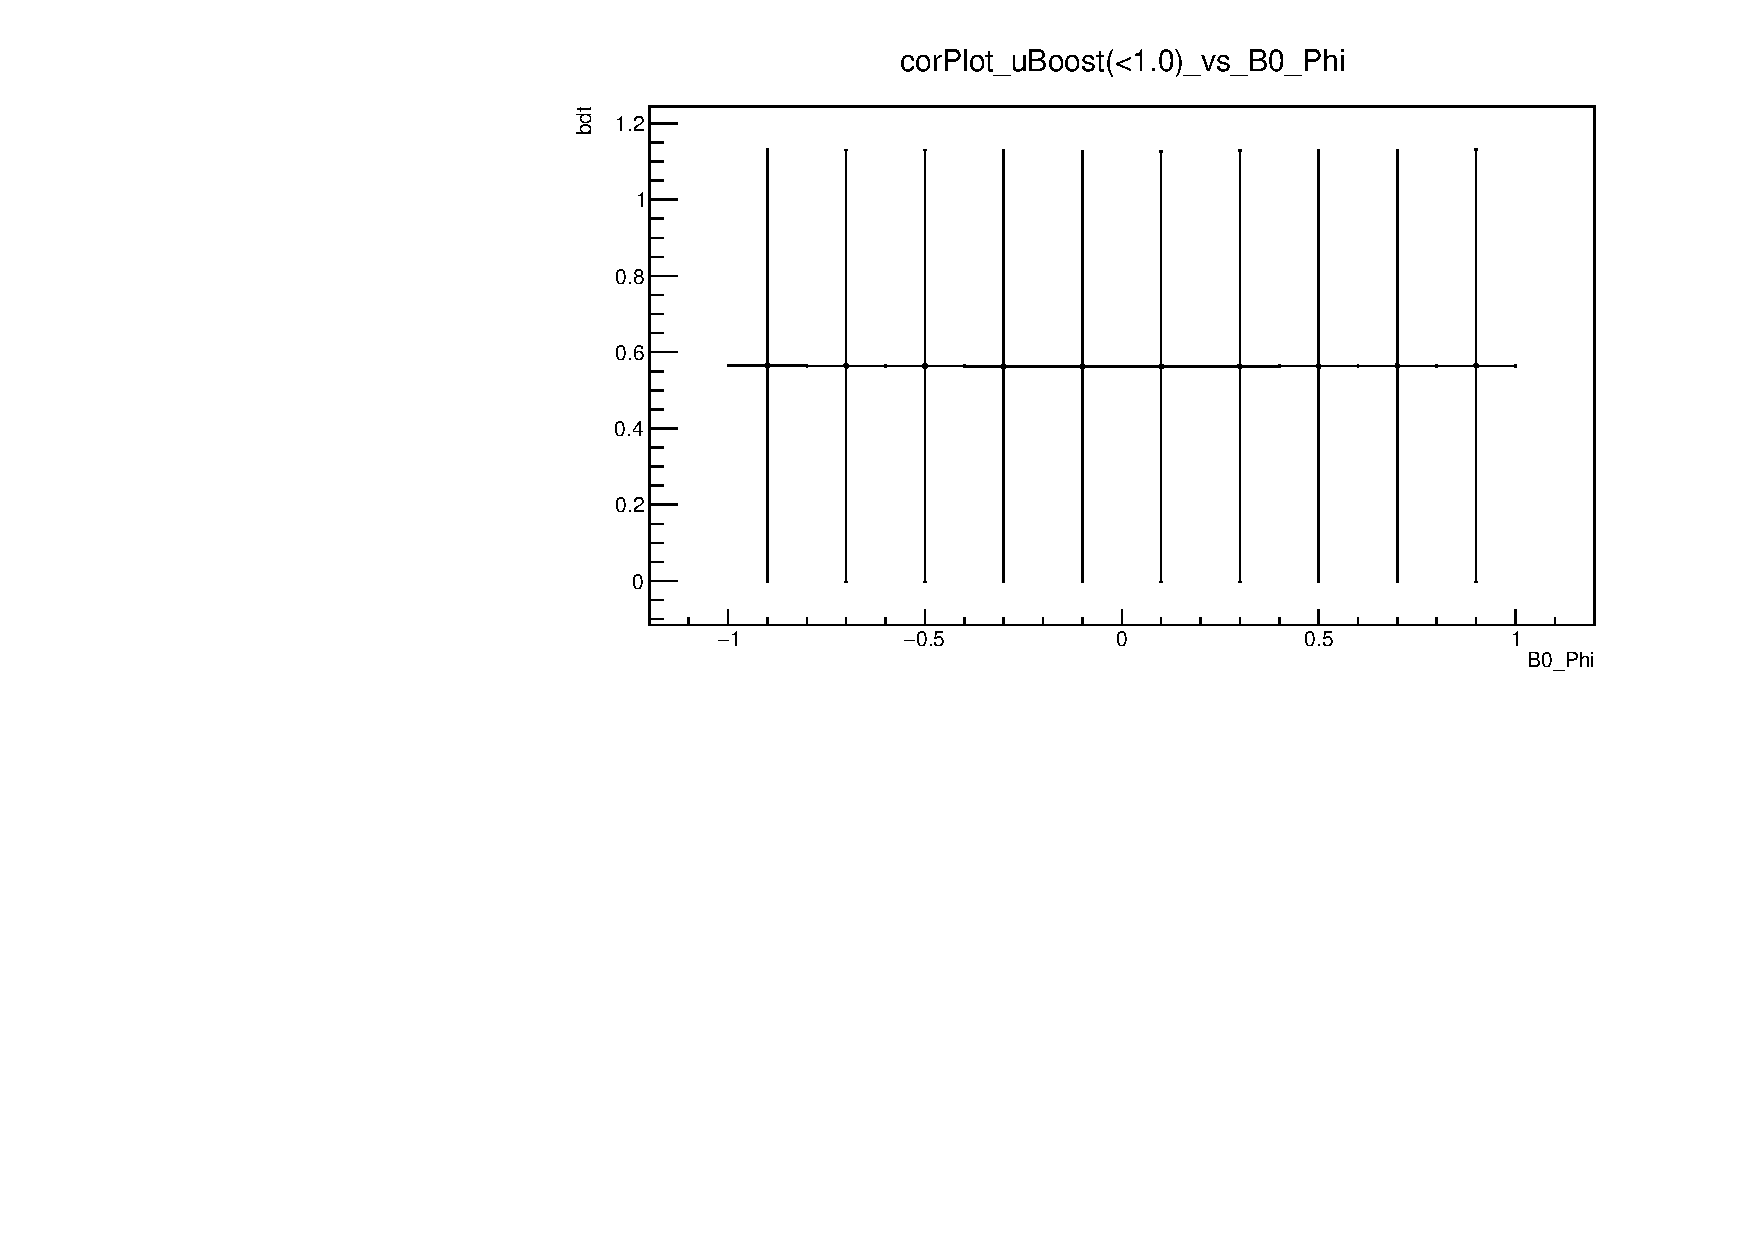
\includegraphics[width=1.0\linewidth]{plots/corPlot_uBoost(<1.0)_vs_B0_Phi.pdf}
\caption{Correlation uBoost VS B0 Phi}
\end{subfigure}
\end{figure}
\end{frame}

% \begin{frame}
%   \frametitle{BDT correlation check}
%
%   \begin{figure}
%   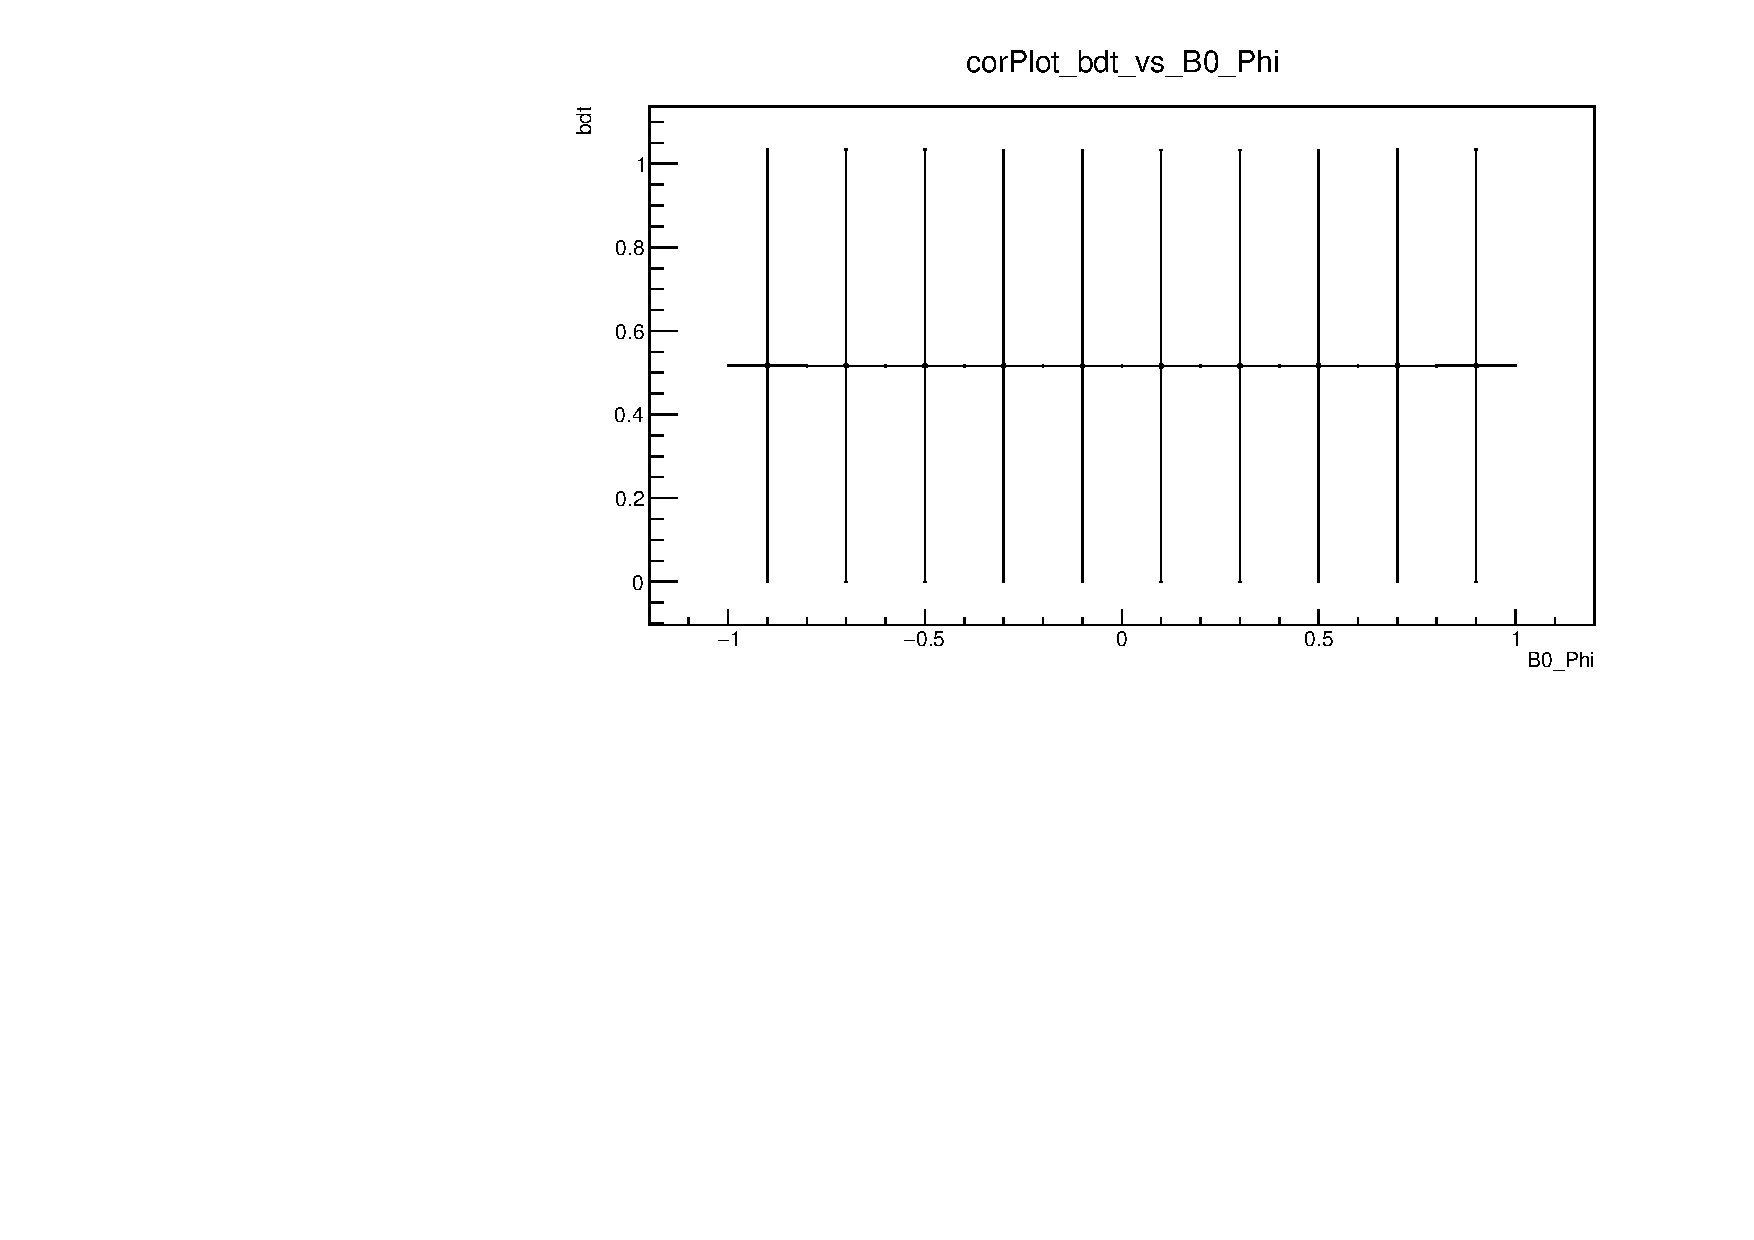
\includegraphics[width=1.0\linewidth]{plots/corPlot_bdt_vs_B0_Phi.pdf}
%   \end{figure}
%
% \end{frame}

\begin{frame}
\frametitle{Roc curves}
The ROC curve gives an estimate how good a bdt performed. There is a roc curve for each of the 10 folds. This is just an example but all the others look similar.
You can see that already at 0.6 true positive rate there is a 0.2 false positive rate. That means that if the bdt got 60\% classified correctly there are already 20\% classified wrongly. This is very bad I am looking into it.
    \begin{figure}
    \centering
    \begin{subfigure}{0.5\textwidth}
    \centering
    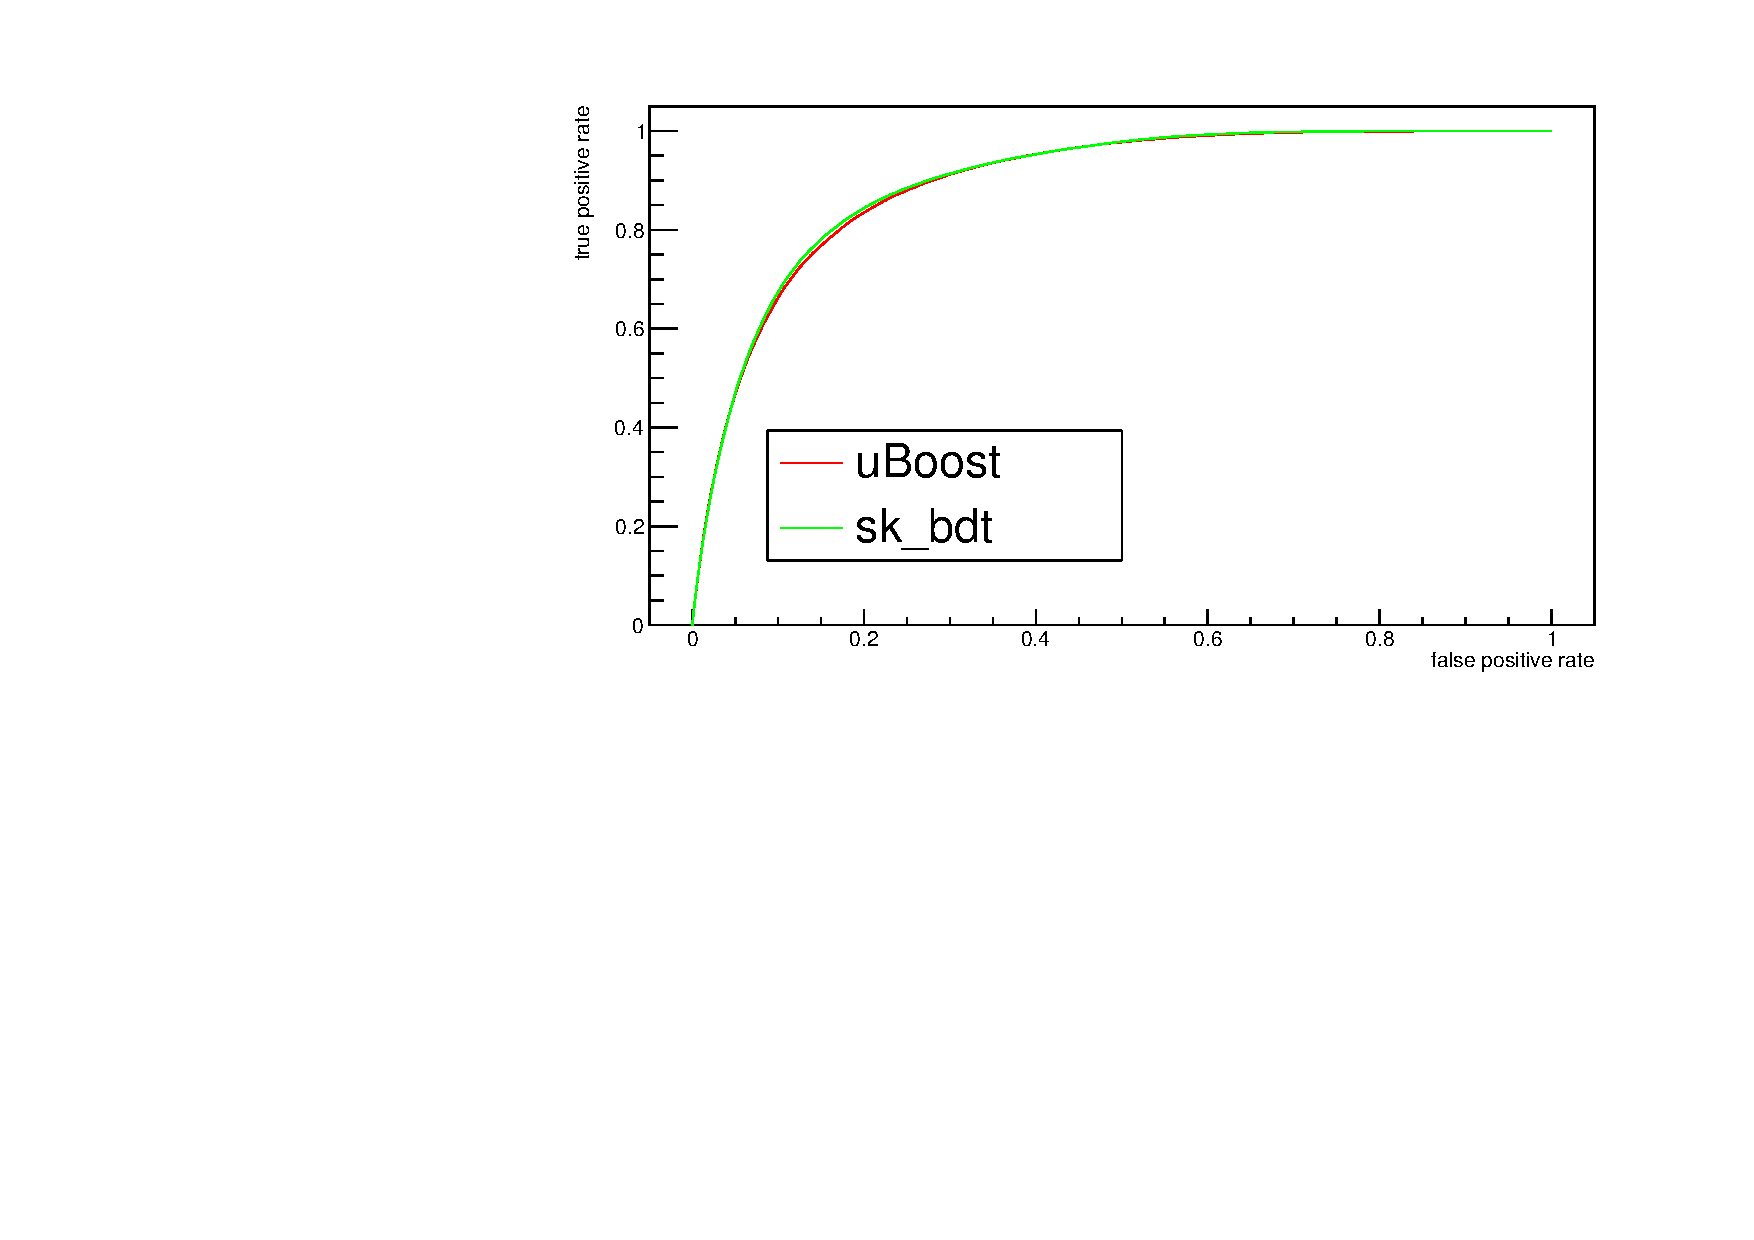
\includegraphics[width=1\linewidth]{roc/fold0_roc}
    \caption{ROC curve of fold 0}
    \end{subfigure}%
    \begin{subfigure}{0.5\textwidth}
    \centering
    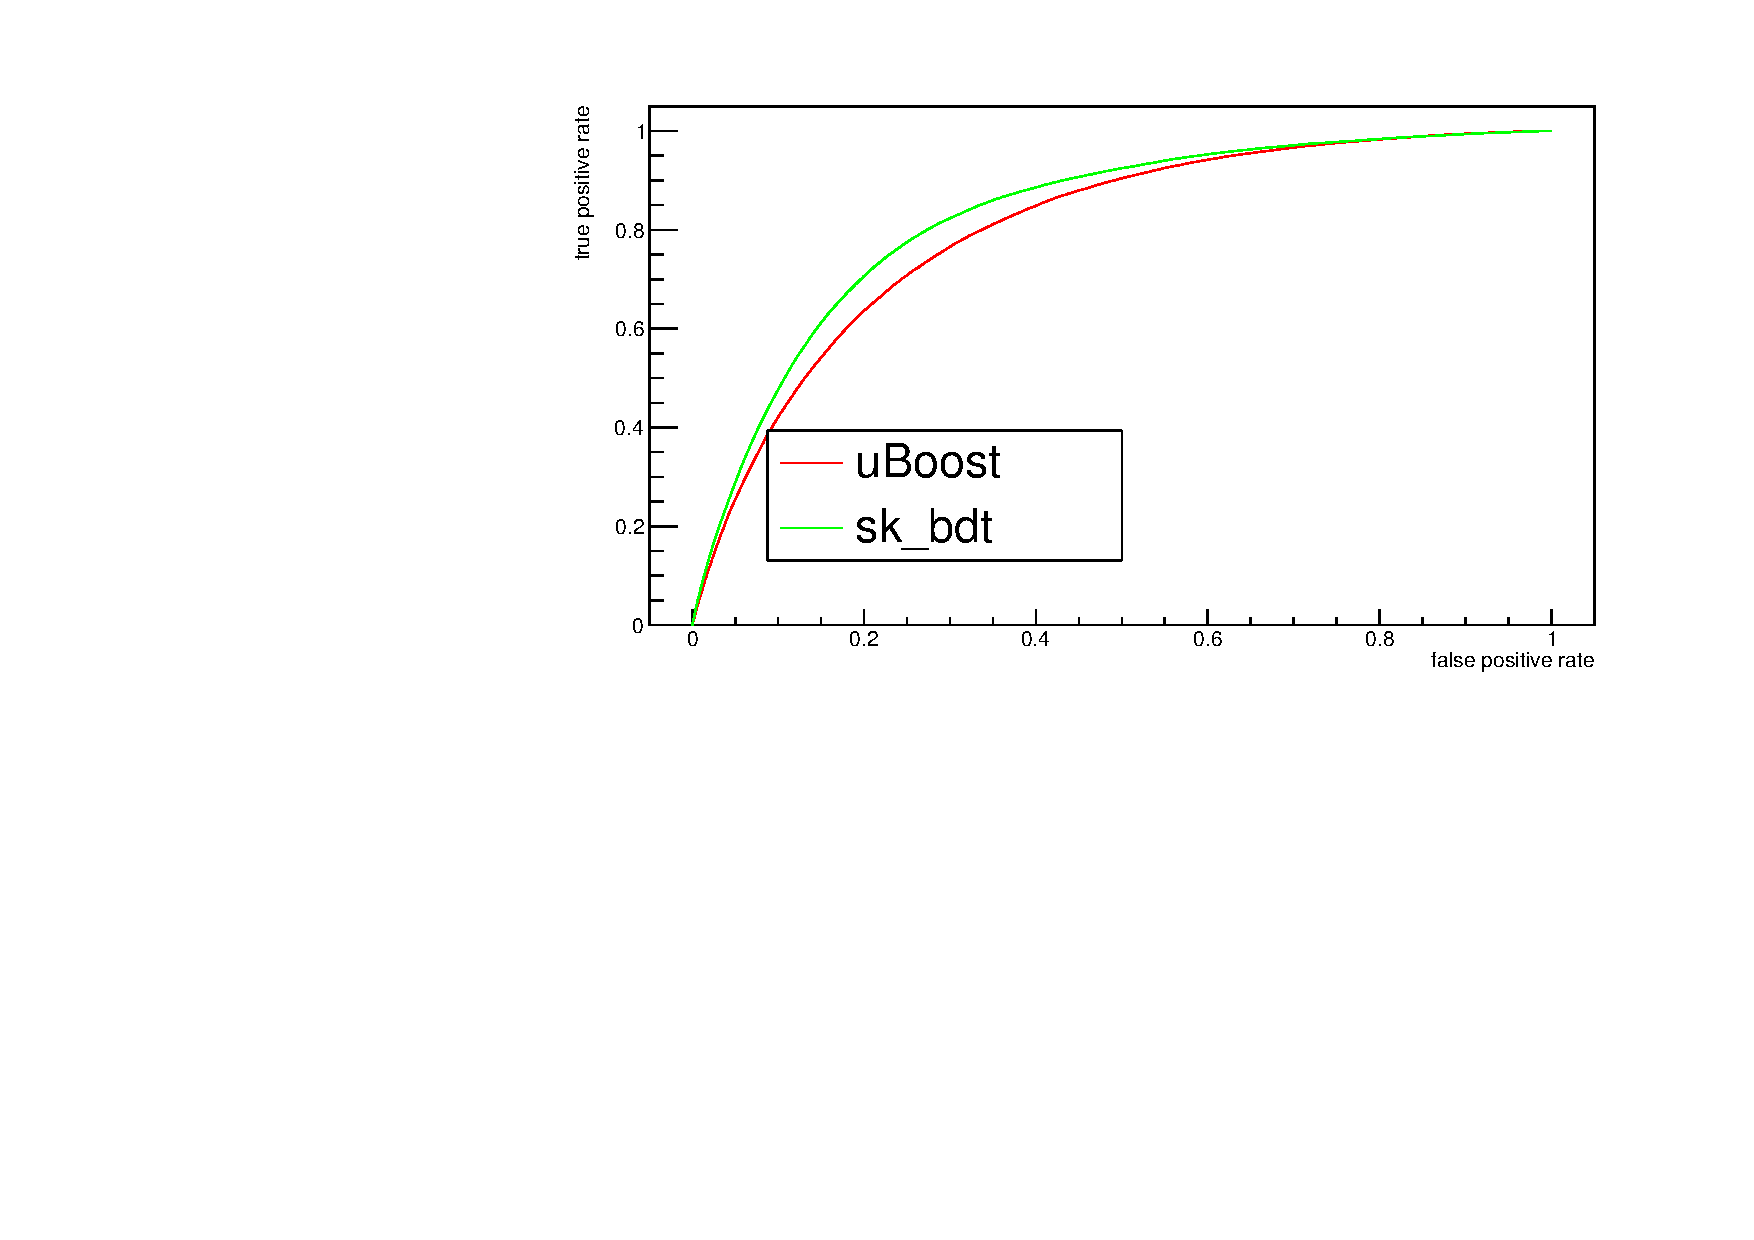
\includegraphics[width=1\linewidth]{roc/fold5_roc}
    \caption{ROC curve of fold 5}
    \end{subfigure}
    \end{figure}

\end{frame}

\begin{frame}
  \frametitle{BDT response histogram}
This are examples of histograms of the bdt responses for one fold.
You can see clearly that most of the data is classified with a 0.5 probability to be signal. There is no information at all in that, this is connected to the bad roc curves above. At the moment I have no idea how to solve that problem. If you have one just write me.
    \begin{figure}
    \centering
    \begin{subfigure}{0.5\textwidth}
    \centering
    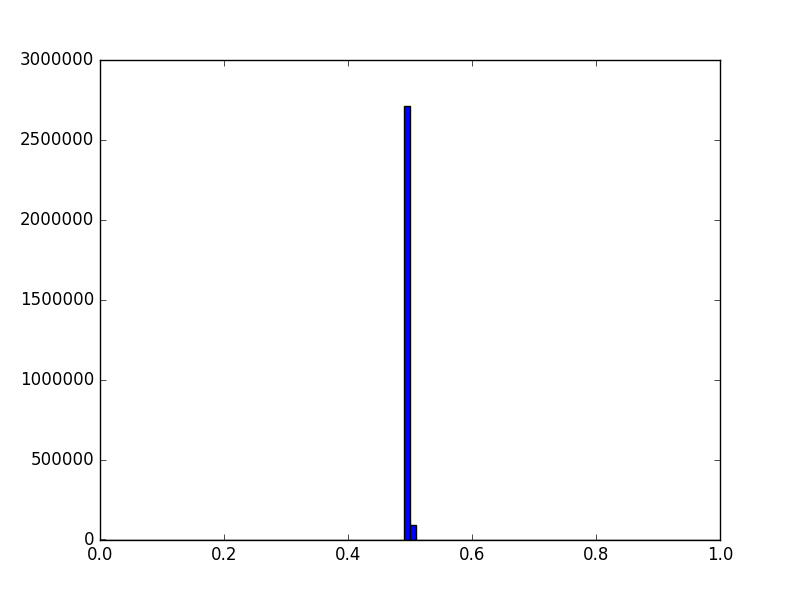
\includegraphics[width=1\linewidth]{plots/sk_bdtHist_fold0}
    \caption{sk bdt response of fold 0}
    \end{subfigure}%
    \begin{subfigure}{0.5\textwidth}
    \centering
    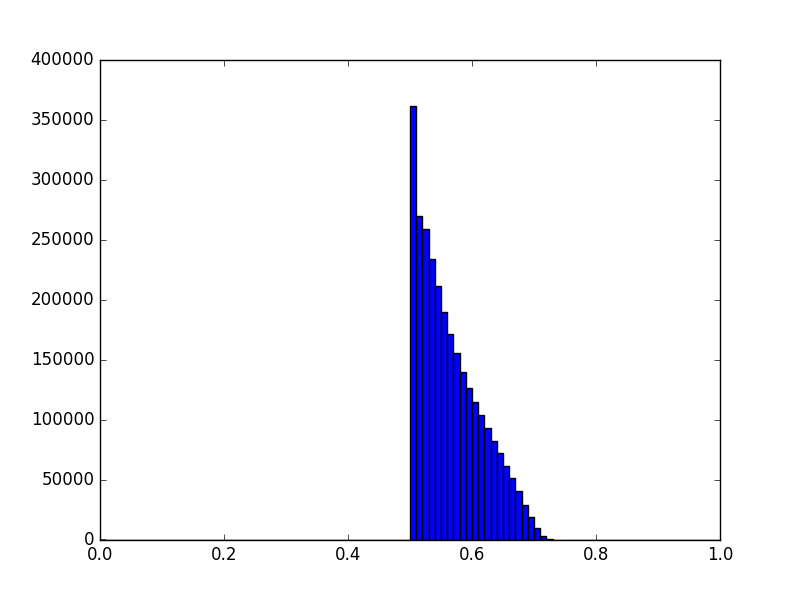
\includegraphics[width=1\linewidth]{plots/uBoostHist_fold0}
    \caption{uBoost response of fold 0}
    \end{subfigure}
    \end{figure}

\end{frame}


%----------------------------------------------------------------------------------------



\end{document}
